%==== KNITR ===================================================================%



%==== START ===================================================================%

\documentclass[10pt]{beamer}\usepackage[]{graphicx}\usepackage[table]{xcolor}
% maxwidth is the original width if it is less than linewidth
% otherwise use linewidth (to make sure the graphics do not exceed the margin)
\makeatletter
\def\maxwidth{ %
  \ifdim\Gin@nat@width>\linewidth
    \linewidth
  \else
    \Gin@nat@width
  \fi
}
\makeatother

\definecolor{fgcolor}{rgb}{0.345, 0.345, 0.345}
\newcommand{\hlnum}[1]{\textcolor[rgb]{0.686,0.059,0.569}{#1}}%
\newcommand{\hlsng}[1]{\textcolor[rgb]{0.192,0.494,0.8}{#1}}%
\newcommand{\hlcom}[1]{\textcolor[rgb]{0.678,0.584,0.686}{\textit{#1}}}%
\newcommand{\hlopt}[1]{\textcolor[rgb]{0,0,0}{#1}}%
\newcommand{\hldef}[1]{\textcolor[rgb]{0.345,0.345,0.345}{#1}}%
\newcommand{\hlkwa}[1]{\textcolor[rgb]{0.161,0.373,0.58}{\textbf{#1}}}%
\newcommand{\hlkwb}[1]{\textcolor[rgb]{0.69,0.353,0.396}{#1}}%
\newcommand{\hlkwc}[1]{\textcolor[rgb]{0.333,0.667,0.333}{#1}}%
\newcommand{\hlkwd}[1]{\textcolor[rgb]{0.737,0.353,0.396}{\textbf{#1}}}%
\let\hlipl\hlkwb

\usepackage{framed}
\makeatletter
\newenvironment{kframe}{%
 \def\at@end@of@kframe{}%
 \ifinner\ifhmode%
  \def\at@end@of@kframe{\end{minipage}}%
  \begin{minipage}{\columnwidth}%
 \fi\fi%
 \def\FrameCommand##1{\hskip\@totalleftmargin \hskip-\fboxsep
 \colorbox{shadecolor}{##1}\hskip-\fboxsep
     % There is no \\@totalrightmargin, so:
     \hskip-\linewidth \hskip-\@totalleftmargin \hskip\columnwidth}%
 \MakeFramed {\advance\hsize-\width
   \@totalleftmargin\z@ \linewidth\hsize
   \@setminipage}}%
 {\par\unskip\endMakeFramed%
 \at@end@of@kframe}
\makeatother

\definecolor{shadecolor}{rgb}{.97, .97, .97}
\definecolor{messagecolor}{rgb}{0, 0, 0}
\definecolor{warningcolor}{rgb}{1, 0, 1}
\definecolor{errorcolor}{rgb}{1, 0, 0}
\newenvironment{knitrout}{}{} % an empty environment to be redefined in TeX

\usepackage{alltt}

\usetheme{Madrid}
\usecolortheme{beaver}

\usepackage[utf8]{inputenc}
\usepackage{amsmath,amssymb}
\usepackage{graphicx}
\usepackage{booktabs}
\usepackage{array}
\usepackage{hyperref}
%\usepackage[round,authoryear]{natbib}
% \setcitestyle{authoryear,round,aysep={, },yysep={; },notesep={, }}

%==== CITATION =====%
\usepackage[round,authoryear]{natbib}
\setcitestyle{authoryear,round,aysep={, },yysep={; },notesep={, }}

%===================%

\usepackage[table]{xcolor}
\usepackage{tikz}
\usetikzlibrary{calc, positioning, arrows.meta}

\definecolor{MainColour}{RGB}{0,72,144}
\definecolor{grey}{RGB}{216,221,227}
\definecolor{darkgrey}{RGB}{149,153,158}
\definecolor{warningRed}{RGB}{145,45,45}

\setbeamercolor{title}{bg=MainColour, fg=white}
\setbeamercolor{frametitle}{bg=MainColour, fg=white}
\setbeamercolor{subtitle}{fg=white}
\setbeamercolor{date in head/foot}{bg=MainColour, fg=white}
\setbeamercolor{footline}{bg=MainColour, fg=white}
\setbeamercolor{block title alerted}{bg=MainColour, fg=white}
\setbeamercolor{block body alerted}{bg=grey, fg=black}
\setbeamercolor{block title}{bg=darkgrey, fg=white}
\setbeamercolor{block body}{bg=grey, fg=black}
\setbeamertemplate{navigation symbols}{}
\setbeamertemplate{caption}[numbered]

\setbeamertemplate{footline}{%
  \leavevmode%
  \hbox{%
    \begin{beamercolorbox}[wd=6.4cm,ht=2.25ex,dp=1ex,leftskip=0.5cm]{date in head/foot}%
      \usebeamerfont{date in head/foot}\insertdate
    \end{beamercolorbox}%
    \begin{beamercolorbox}[wd=6.4cm,ht=2.25ex,dp=1ex]{date in head/foot}%
      \usebeamerfont{date in head/foot}\hfill\insertframenumber\hspace*{0.75cm}%
    \end{beamercolorbox}}%
  \vskip0pt%
}

\newcolumntype{L}[1]{>{\raggedright\arraybackslash}p{#1}}
\newcolumntype{R}[1]{>{\raggedleft\arraybackslash}p{#1}}
\newcommand{\sourcefoot}[1]{\vspace{0.25em}{\tiny \textit{Source:} #1}}
\newcommand{\remarkfoot}[1]{\vspace{0.25em}{\tiny \textit{Remark:} #1}}

\newcommand{\status}[1]{\textcolor{warningRed}{\textbf{#1}}}

%==== Abbreviations ====%
\newcommand{\dyn}{\texttt{dynamic\_csi}}
\newcommand{\perm}{\texttt{permanent\_csi}}
\newcommand{\agbase}{AG Base Dataset}
\newcommand{\agexp}{AG Expanded Dataset}
\newcommand{\aglatent}{AG Latent Dataset (VAE)}
\newcommand{\agvae}{AG Exp. Dataset + VAE}
\graphicspath{{../../../03_Output/Figures/}}

%==== COLORS ===========%

\definecolor{posgreen}{RGB}{15,110,86}    % strategy / positive
\definecolor{posgreenL}{RGB}{29,158,117}  % second bar series
\definecolor{lightblue}{RGB}{181,212,244} % range bars
\definecolor{negred}{RGB}{163,45,45}      % negative contribution

%==== Title Slide ====%
\title[The Agony and the Ecstasy]{The Agony and the Ecstasy}
\subtitle{Constructing a ``Crash-Filtered'' Equity Index using Machine Learning}
\author{Tristan Leiter}
\institute[WU]{Vienna University of Business and Economics \\
        \medskip
        \scriptsize Supervisor: Prof. Kurt Hornik}
\date{June 2nd, 2026}

%==== DOCUMENT ================================================================%

\IfFileExists{upquote.sty}{\usepackage{upquote}}{}
\begin{document}

\begin{frame}
  \titlepage
\end{frame}

%==== 1. MOTIVATION ===========================================================%

\section{Motivation}
\begin{frame}{The Agony and Ecstasy}
\small
\begin{alertblock}{Passive indices are exposed to both extremes}
Long-run index returns are driven by a few high-performing stocks, while a considerable share of constituents suffer catastrophic declines.
% Cembalest JPM paper.
\end{alertblock}

\vspace{0.35em}
\begin{columns}[t]
\begin{column}{0.48\textwidth}
\textbf{Ecstasy}
\begin{itemize}
  \item Extreme winners carry a large share of long-run wealth creation.
  \item Winners can be volatile, expensive, or distressed.
  \item Thus, even a small amount of disregarded winners can hurt performance.
\end{itemize}
\end{column}
\begin{column}{0.48\textwidth}
\textbf{Agony}
\begin{itemize}
  \item Some constituents experience deep and persistent drawdowns without recovery.
  \item Passive strategies may hold imploding firms for too long.
\end{itemize}
\end{column}
\end{columns}

\vspace{0.35em}
\begin{block}{Solution}
\scriptsize
The challenge is not to eliminate highly volatile stocks. It is to distinguish recoverable volatility from persistent implosion. The empirical question is whether catastrophically declining firms are forecastable using ideas from credit-risk modelling, but with market-based distress signals.
\end{block}
%\sourcefoot{Motivation follows Cembalest (2014) and the CSI framing in Tewari et al. (2024).}
\end{frame}

%==== 2. RESEARCH QUESTION ====================================================%

\section{Research Question}
\begin{frame}{Research Question}
\small
\textbf{Main research question}
\begin{alertblock}{}
To what extent does a ``Crash-Filtered'' equity index, constructed via probabilistic implosion modeling, generate superior risk-adjusted returns compared to the market benchmark and traditional minimum-volatility strategies?
\end{alertblock}

The probabilistic implosion model follows the Catastrophic Stock Implosion approach proposed by Tewari et al. (2024). Instead of relying only on formal bankruptcy declarations, CSI uses market-based price-path signals.

\vspace{0.35em}

\textbf{Subquestions:}

  \begin{itemize}
      \setlength\itemsep{0.3em}
    \item How does the integration of Autoencoders for feature engineering impact the Average Precision of Ensemble models compared to those trained solely on raw financial data?

%%% RQ 2:
    % \item Do Ensemble methods exhibit a superior ability to distinguish between recoverable volatility ('Ecstasy') and terminal implosion ('Agony') compared to indiscriminate volatility-based exclusion strategies?
    \item To what extent do Ensemble methods reduce the False Positive Rate (classifying recoverable volatility as CSI) compared to traditional volatility-based exclusion strategies, while maintaining Recall?

%%% RQ 3:
    \item Which features are most important for distinguishing between "Zombie" firms (CSI) and non-zombie firms?

  \end{itemize}


\end{frame}

%==== 3. DATASET ==============================================================%

\section{Dataset}
\begin{frame}{Dataset}
\small

\begin{alertblock}{Empirical design}
\scriptsize
The final panel keeps only observable CRSP firm-years: each row has the required monthly return and market-cap scaffold. Temporary and permanent CSI use the same 188,460-row scaffold; unresolved $y=\mathrm{NA}$ rows are retained in the panel but excluded from supervised model metrics.
\end{alertblock}

\vspace{0.4em}

\begin{center}
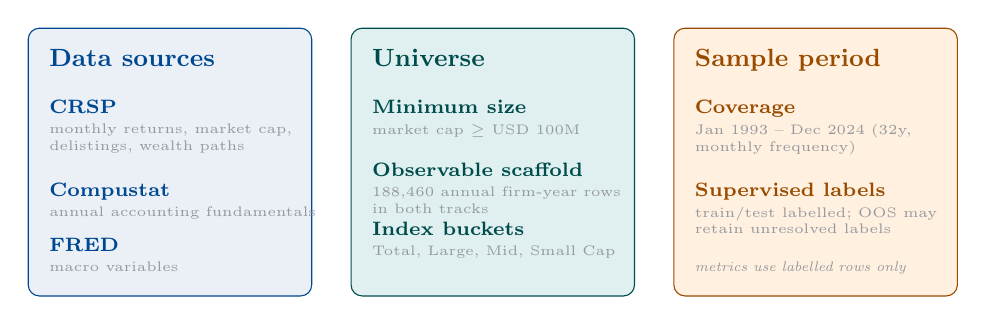
\begin{tikzpicture}[
  font=\scriptsize,
  card/.style={draw, rounded corners=4pt, minimum width=3.6cm, minimum height=3.4cm, anchor=north west, inner sep=6pt, align=left},
  cardA/.style={card, fill=MainColour!8, draw=MainColour},
  cardB/.style={card, fill=teal!12, draw=teal!60!black},
  cardC/.style={card, fill=orange!12, draw=orange!60!black},
  cardtitle/.style={font=\small\bfseries},
  fieldlabel/.style={font=\scriptsize\bfseries},
  fieldbody/.style={font=\tiny, text=darkgrey}
]
% Card A: Data sources
\node[cardA] (a) at (0,0) {};
\node[cardtitle, anchor=north west, MainColour] at (0.15,-0.15) {Data sources};
\node[fieldlabel, anchor=north west, MainColour] at (0.15,-0.8) {CRSP};
\node[fieldbody, anchor=north west, text width=3.4cm] at (0.15,-1.1) {monthly returns, market cap, delistings, wealth paths};
\node[fieldlabel, anchor=north west, MainColour] at (0.15,-1.85) {Compustat};
\node[fieldbody, anchor=north west, text width=3.4cm] at (0.15,-2.15) {annual accounting fundamentals};
\node[fieldlabel, anchor=north west, MainColour] at (0.15,-2.55) {FRED};
\node[fieldbody, anchor=north west, text width=3.4cm] at (0.15,-2.85) {macro variables};

% Card B: Universe
\node[cardB] (b) at (4.1,0) {};
\node[cardtitle, anchor=north west, teal!60!black] at (4.25,-0.15) {Universe};
\node[fieldlabel, anchor=north west, teal!60!black] at (4.25,-0.8) {Minimum size};
\node[fieldbody, anchor=north west, text width=3.4cm] at (4.25,-1.1) {market cap $\geq$ USD 100M};
\node[fieldlabel, anchor=north west, teal!60!black] at (4.25,-1.6) {Observable scaffold};
\node[fieldbody, anchor=north west, text width=3.4cm] at (4.25,-1.9) {188,460 annual firm-year rows in both tracks};
\node[fieldlabel, anchor=north west, teal!60!black] at (4.25,-2.35) {Index buckets};
\node[fieldbody, anchor=north west, text width=3.4cm] at (4.25,-2.65) {Total, Large, Mid, Small Cap};

% Card C: Sample period
\node[cardC] (c) at (8.2,0) {};
\node[cardtitle, anchor=north west, orange!60!black] at (8.35,-0.15) {Sample period};
\node[fieldlabel, anchor=north west, orange!60!black] at (8.35,-0.8) {Coverage};
\node[fieldbody, anchor=north west, text width=3.4cm] at (8.35,-1.1) {Jan 1993 -- Dec 2024 (32y, monthly frequency)};
\node[fieldlabel, anchor=north west, orange!60!black] at (8.35,-1.85) {Supervised labels};
\node[fieldbody, anchor=north west, text width=3.4cm] at (8.35,-2.15) {train/test labelled; OOS may retain unresolved labels};
\node[fieldbody, anchor=north west, text width=3.4cm, font=\tiny\itshape] at (8.35,-2.85) {metrics use labelled rows only};
\end{tikzpicture}
\end{center}

\vspace{0.3em}

\textbf{Temporal split}

\vspace{0.25em}
\begin{center}
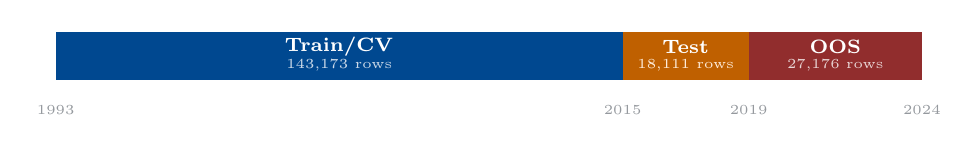
\begin{tikzpicture}[font=\scriptsize]
% Year axis
\foreach \x/\year in {0/1993, 7.2/2015, 8.8/2019, 11.0/2024} {
  \node[anchor=north, darkgrey] at (\x,-0.2) {\tiny\year};
}

% Bars
\fill[MainColour]      (0.0,0.0) rectangle (7.2,0.6);
\node[white] at (3.6,0.42) {\textbf{Train/CV}};
\node[MainColour!20] at (3.6,0.18) {\tiny 143,173 rows};

\fill[orange!75!black] (7.2,0.0) rectangle (8.8,0.6);
\node[white] at (8.0,0.42) {\textbf{Test}};
\node[orange!15] at (8.0,0.18) {\tiny 18,111 rows};

\fill[warningRed]      (8.8,0.0) rectangle (11.0,0.6);
\node[white] at (9.9,0.42) {\textbf{OOS}};
\node[warningRed!20] at (9.9,0.18) {\tiny 27,176 rows};
\end{tikzpicture}
\end{center}

\end{frame}

%==== 5. RESPONSE VARIABLE ====================================================%

\section{Response Variable}
\begin{frame}{Methodology I: Response Variable Classification}
\small
Following Tewari et al. (2024), a stock is classified as a CSI candidate if it satisfies all three path criteria:

\vspace{0.3em}
\begin{itemize}
  \setlength\itemsep{0.4em}
  \item \textbf{Initial Crash ($C$):} more than a $C$ drawdown from the trailing peak marks the beginning of the ``zombie'' period.  \hfill \textcolor{warningRed}{\small $C \leq -80\%$}
  \item \textbf{Non-Recovery ($M$):} maximum cumulative return remains below the recovery ceiling $M$ during the zombie period. \hfill \textcolor{warningRed}{\small $M \leq -20\%$}
  \item \textbf{Zombie Period ($T$):} duration of the confirmation window during which non-recovery must hold. \hfill \textcolor{warningRed}{\small $T = 18$ months}
\end{itemize}

\vspace{0.35em}
The prediction task is annual. A trigger in calendar year $t+1$ gives the firm-year observation at $t$ a positive label when the track-specific confirmation rule is met:
\begin{equation*}
y_{i,t} =
\begin{cases}
1, & \text{if stock } i \text{ triggers a qualifying CSI event within } [t,t+h],\\
0, & \text{otherwise}.
\end{cases}
\end{equation*}

\end{frame}

%==== 6. Applying the classification ==========================================%

\begin{frame}{Applying the paper classification}

\small
By strictly applying the methodology proposed by \citet{Tewari2024},
one finds 8,517 response observations for the selected CRSP-dataset within the 1993 to 2024
time period. The prevalence of the response variable is similar across the Train and
Test datasets. Overall, the whole dataset has 188,460 observations, with roughly
75\% being clustered in the Train set.


\vspace{0.2em}
\begin{table}[ht]
\centering
\scriptsize
\setlength{\tabcolsep}{4.4pt}
\begin{tabular}{L{1.7cm}R{1.25cm}R{1.1cm}R{1.1cm}R{1.25cm}R{1.0cm}}
\toprule
Split & Obs. rows & $y=0$ & $y=1$ & Labelled & Prev. \\
\midrule
Full & 188,460 & 171,269 & \textbf{8,517} & 179,786 & 4.74\% \\
Train & 143,173 & 136,630 & 6,543 & 143,173 & 4.57\% \\
Test & 18,111 & 17,307 & 804 & 18,111 & 4.44\% \\
OOS & 27,176 & 17,332 & 1,170 & 18,502 & 6.32\% \\
\bottomrule
\end{tabular}
\end{table}

\vspace{0.15em}
\begin{alertblock}{Motivation for robustness}
\scriptsize
Even though the paper outlines that a combination of classification grid-values were tested,
the selected combination still appears arbitary. For this reason, further robustness checks
will be conducted to evaluate the chosen grid-values. It will be asked whether the dataset actually contains
the bankrupt firms and how different the prevalence-rate of the response variable is when testing different
grid-combinations.
\end{alertblock}
\end{frame}

%==== 7. Robustness I =========================================================%

\begin{frame}{Robustness I: Do CSI-firms go bankrupt?}

\textbf{Validation question:} Among firms that eventually delist or bankrupt, how many had already been classified as CSI?

\vspace{0.25em}
\begin{table}[ht]
\centering
\scriptsize
\setlength{\tabcolsep}{2.5pt}
\begin{tabular}{L{3.15cm}R{1.2cm}R{1.0cm}R{1.45cm}R{1.0cm}R{1.0cm}R{1.35cm}}
\toprule
Scenario & CSI rows & CSI firms & CRSP 572-574 firms & Detected & Missed & Detection rate \\
\midrule
Before: \texttt{confirmed\_csi} only & 8,369 & 5,642 & 629 & 151 & 478 & 24.0\% \\
\bottomrule
\end{tabular}
\end{table}

\vspace{0.35em}

{\scriptsize CRSP bankruptcy-related delisting codes 572, 573, and 574 are used as the terminal-distress audit set.}

\vspace{0.45em}

\textbf{Core issue:} The low-detection rate causes methodological issues. If one sticks strictly to the paper,
then the CSI methodology should catch firms which do not recover anymore. Yet, the data shows a different result.


\end{frame}

%==== 8. Methodology II =======================================================%

\begin{frame}{Methodology II: ``Temporary-CSI''}
\small

\begin{alertblock}{Revisions to the classification methodology}
\scriptsize
The original CSI-classification grid remains unchanged. It is proposed to explicitly add all
firms, which match the CRSP-codes 572,573 and 574, to the dataset after observing
a valid drawdown trigger. This classification methodology will henceforth be referred to
as "Temporary-CSI".
\end{alertblock}

\vspace{0.4em}

\begin{center}
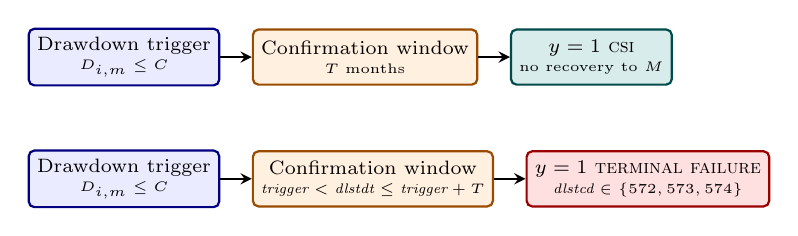
\begin{tikzpicture}[
  font=\scriptsize,
  node distance=4mm,
  box/.style={draw, rounded corners=2pt, minimum height=7mm, inner sep=3pt, align=center},
  csi/.style={box, fill=blue!8,  draw=blue!50!black},
  win/.style={box, fill=orange!12, draw=orange!60!black},
  csiy/.style={box, fill=teal!15, draw=teal!60!black},
  bkyy/.style={box, fill=red!12,  draw=red!60!black},
  ->, >=stealth, thick
]
% Row 1: original CSI rule
\node[csi]               (t1) {Drawdown trigger\\[-1pt]\tiny $D_{i,m}\leq C$};
\node[win,  right=of t1] (w1) {Confirmation window\\[-1pt]\tiny $T$ months};
\node[csiy, right=of w1] (y1) {$y=1$ \textsc{csi}\\[-1pt]\tiny no recovery to $M$};
\draw (t1) -- (w1);
\draw (w1) -- (y1);

% Row 2: added terminal-failure path
\node[csi,  below=8mm of t1] (t2) {Drawdown trigger\\[-1pt]\tiny $D_{i,m}\leq C$};
\node[win,  right=of t2]     (w2) {Confirmation window\\[-1pt]\tiny $\textit{trigger}<\textit{dlstdt}\leq\textit{trigger}+T$};
\node[bkyy, right=of w2]     (y2) {$y=1$ \textsc{terminal failure}\\[-1pt]\tiny $\textit{dlstcd}\in\{572,573,574\}$};
\draw (t2) -- (w2);
\draw (w2) -- (y2);
\end{tikzpicture}
\end{center}

\vspace{0.4em}

\begin{table}[ht]
\centering
\scriptsize
\setlength{\tabcolsep}{4pt}
\begin{tabular}{lrrrr}
\toprule
Scenario & Bankrupting & Detected & Missed & \textbf{Detection} \\
\midrule
Before: \texttt{CSI} only            & 629 & 151 & 478 & 24.0\% \\
After:  \texttt{CSI} + terminal failure & 629 & \textbf{545} & 84 & \textbf{86.65\%} \\
\bottomrule
\end{tabular}
\end{table}

\vspace{-0.2em}
{\tiny\color{darkgrey} The 84 remaining misses are treated as methodological exclusions under the retained CSI-trigger rule, not as known pipeline errors.}
\end{frame}

%==== 9. Robustness II ========================================================%

\begin{frame}{Robustness II: Do CSI-classified firms recover again?}
\vspace{0.15em}
{\small\textbf{In addition to bankruptcy checks, robustness checks were also conducted to
determine whether CSI-classified firms are in persistent decline.}}

{\scriptsize A grid-search for the three classification paramaters was conducted to track the
five-year recovery of firms after classification. Subsequently, each firm is sorted into one
of five buckets depending on its five-year performance after classification.}

\vspace{0.2em}

\begin{center}
\resizebox{0.98\textwidth}{!}{%
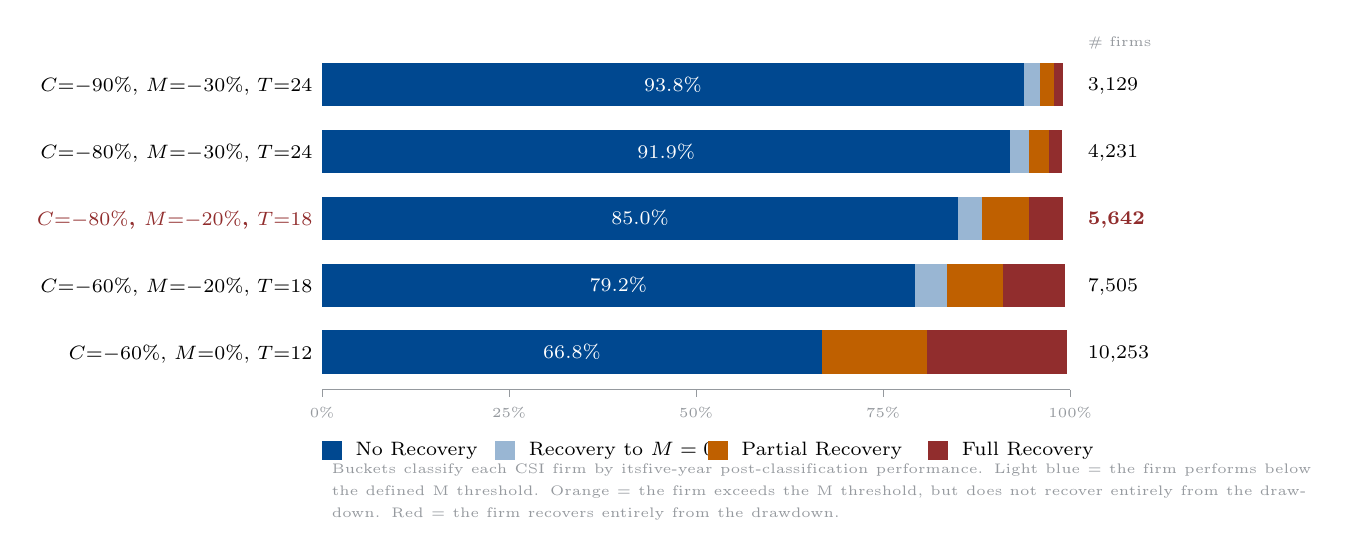
\begin{tikzpicture}[
  font=\scriptsize,
  bar/.style={draw=none},
  baseframe/.style={draw=warningRed, dashed, thick, rounded corners=2pt},
]
% Axis: 0..100 in tikz units = 9.5cm
\def\barH{0.55}      % bar height in cm
\def\rowSep{0.85}    % vertical distance between rows
\def\barX{3.6}       % bar left edge (after row label)
\def\barW{9.5}       % bar width = 100%

% Header for the right-hand-side count column
\node[anchor=west, darkgrey] at (\barX+\barW+0.1,7.25){\tiny \# firms};

% Row 1: C-90 M-30 T24 — 93.8 / 2.2 / 1.9 / 1.2 — 3,129 firms
\node[anchor=east] at (\barX,6.7){$C{=}{-}90\%$, $M{=}{-}30\%$, $T{=}24$};
\node[anchor=west] at (\barX+\barW+0.1,6.7){3,129};
\fill[MainColour]      (\barX,6.45)                              rectangle ++(\barW*0.938,\barH);
\fill[MainColour!40]   (\barX+\barW*0.938,6.45)                  rectangle ++(\barW*0.022,\barH);
\fill[orange!75!black] (\barX+\barW*0.960,6.45)                  rectangle ++(\barW*0.019,\barH);
\fill[warningRed]      (\barX+\barW*0.979,6.45)                  rectangle ++(\barW*0.012,\barH);
\node[white] at (\barX+\barW*0.469,6.725){93.8\%};

% Row 2: C-80 M-30 T24 — 91.9 / 2.6 / 2.7 / 1.7 — 4,231 firms
\node[anchor=east] at (\barX,5.85){$C{=}{-}80\%$, $M{=}{-}30\%$, $T{=}24$};
\node[anchor=west] at (\barX+\barW+0.1,5.85){4,231};
\fill[MainColour]      (\barX,5.60)                              rectangle ++(\barW*0.919,\barH);
\fill[MainColour!40]   (\barX+\barW*0.919,5.60)                  rectangle ++(\barW*0.026,\barH);
\fill[orange!75!black] (\barX+\barW*0.945,5.60)                  rectangle ++(\barW*0.027,\barH);
\fill[warningRed]      (\barX+\barW*0.972,5.60)                  rectangle ++(\barW*0.017,\barH);
\node[white] at (\barX+\barW*0.460,5.875){91.9\%};

% Row 3: BASE — C-80 M-20 T18 — 85.0 / 3.2 / 6.3 / 4.6 — 5,642 firms
\node[anchor=east, warningRed] at (\barX,5.0){\textbf{$C{=}{-}80\%$, $M{=}{-}20\%$, $T{=}18$}};
\node[anchor=west, warningRed] at (\barX+\barW+0.1,5.0){\textbf{5,642}};
\fill[MainColour]      (\barX,4.75)                              rectangle ++(\barW*0.850,\barH);
\fill[MainColour!40]   (\barX+\barW*0.850,4.75)                  rectangle ++(\barW*0.032,\barH);
\fill[orange!75!black] (\barX+\barW*0.882,4.75)                  rectangle ++(\barW*0.063,\barH);
\fill[warningRed]      (\barX+\barW*0.945,4.75)                  rectangle ++(\barW*0.046,\barH);
\node[white] at (\barX+\barW*0.425,5.025){85.0\%};

% Row 4: C-60 M-20 T18 — 79.2 / 4.4 / 7.4 / 8.3 — 7,505 firms
\node[anchor=east] at (\barX,4.15){$C{=}{-}60\%$, $M{=}{-}20\%$, $T{=}18$};
\node[anchor=west] at (\barX+\barW+0.1,4.15){7,505};
\fill[MainColour]      (\barX,3.90)                              rectangle ++(\barW*0.792,\barH);
\fill[MainColour!40]   (\barX+\barW*0.792,3.90)                  rectangle ++(\barW*0.044,\barH);
\fill[orange!75!black] (\barX+\barW*0.836,3.90)                  rectangle ++(\barW*0.074,\barH);
\fill[warningRed]      (\barX+\barW*0.910,3.90)                  rectangle ++(\barW*0.083,\barH);
\node[white] at (\barX+\barW*0.396,4.175){79.2\%};

% Row 5: C-60 M-0 T12 — 66.8 / 0.0 / 14.1 / 18.7 — 10,253 firms
\node[anchor=east] at (\barX,3.30){$C{=}{-}60\%$, $M{=}0\%$, $T{=}12$};
\node[anchor=west] at (\barX+\barW+0.1,3.30){10,253};
\fill[MainColour]      (\barX,3.05)                              rectangle ++(\barW*0.668,\barH);
\fill[orange!75!black] (\barX+\barW*0.668,3.05)                  rectangle ++(\barW*0.141,\barH);
\fill[warningRed]      (\barX+\barW*0.809,3.05)                  rectangle ++(\barW*0.187,\barH);
\node[white] at (\barX+\barW*0.334,3.325){66.8\%};

% Axis ticks
\draw[darkgrey, thin] (\barX,2.85) -- (\barX+\barW,2.85);
\foreach \p/\l in {0/0\%, 0.25/25\%, 0.5/50\%, 0.75/75\%, 1.0/100\%} {
  \draw[darkgrey, thin] (\barX+\barW*\p,2.85) -- (\barX+\barW*\p,2.75);
  \node[anchor=north, darkgrey] at (\barX+\barW*\p,2.75){\tiny\l};
}

% Legend (below the chart)
\def\legY{1.95}
\def\legTextY{2.075}

\fill[MainColour]      (\barX+0.00,\legY) rectangle ++(0.25,0.25);
\node[anchor=west] at (\barX+0.30,\legTextY){No Recovery};

\fill[MainColour!40]   (\barX+2.20,\legY) rectangle ++(0.25,0.25);
\node[anchor=west] at (\barX+2.50,\legTextY){Recovery to $M=0$};

\fill[orange!75!black] (\barX+4.90,\legY) rectangle ++(0.25,0.25);
\node[anchor=west] at (\barX+5.20,\legTextY){Partial Recovery};

\fill[warningRed]      (\barX+7.70,\legY) rectangle ++(0.25,0.25);
\node[anchor=west] at (\barX+8.00,\legTextY){Full Recovery};

\node[anchor=west, darkgrey, text width=12.5cm] at (\barX,1.55)
{\tiny Buckets classify each CSI firm by itsfive-year post-classification performance.
Light blue = the firm performs below the defined M threshold. Orange  = the firm exceeds the
M threshold, but does not recover entirely from the drawdown. Red = the firm recovers entirely
from the drawdown.};

\end{tikzpicture}
}
\end{center}

\end{frame}


%==== 10. Methodology III =====================================================%

\begin{frame}{Methodology III: ``Permanent-CSI''}
\scriptsize

\begin{alertblock}{Dealing with recovering firms}
\scriptsize
To deal with the prior outlined false-positives due to observing a non-neglectible portion of
recovering firms, it is proposed to test a secondary classification methodology: "Permanent-CSI".
This methodology is even further forward looking, if a firm did not recover above the defined
M threshold after 5 years, it will be classified as a CSI-event.
\end{alertblock}

\vspace{0.1em}

\begin{center}
\hspace*{0cm}%
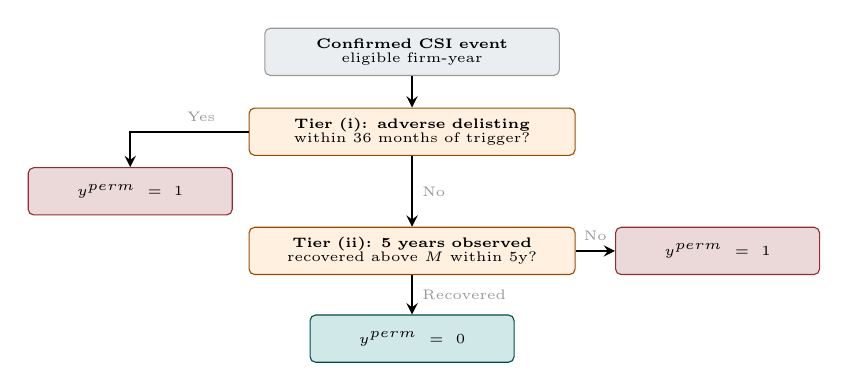
\begin{tikzpicture}[
  font=\tiny,
  node distance=3mm,
  csibox/.style={draw, rounded corners=2pt, minimum height=6mm, inner sep=2pt, align=center},
  csientry/.style={csibox, fill=grey!50, draw=darkgrey, text width=3.6cm},
  csicheck/.style={csibox, fill=orange!12, draw=orange!60!black, text width=4.0cm},
  csipos/.style={csibox, fill=warningRed!18, draw=warningRed, text width=2.45cm},
  csineg/.style={csibox, fill=teal!18, draw=teal!60!black, text width=2.45cm},
  csiedge/.style={->, >=stealth, thick},
  nolab/.style={right, font=\tiny, text=darkgrey},
  altlab/.style={font=\tiny, text=darkgrey}
]
% Top: entry event
\node[csientry] (entry) {\textbf{Confirmed CSI event}\\[-1pt]\tiny eligible firm-year};

% Tier (i)
\node[csicheck, below=4mm of entry] (t1) {\textbf{Tier (i): adverse delisting}\\[-1pt]\tiny within 36 months of trigger?};

% Tier (ii)
\node[csicheck, below=9mm of t1] (t2) {\textbf{Tier (ii): 5 years observed}\\[-1pt]\tiny recovered above $M$ within 5y?};

% Single left-side red outcome — placed between the two tiers, offset left
\coordinate (midy) at ($(t1.south)!0.5!(t2.north)$);
\node[csipos, anchor=east] at ([xshift=-2mm]t1.west |- midy) (term) {$y^{perm}=1$};

% Right-side outcome — same height as Tier (ii)
\node[csipos, right=5mm of t2] (dur) {$y^{perm}=1$};

% Below Tier (ii) — Recovered branch
\node[csineg, below=5mm of t2] (recov) {$y^{perm}=0$};

% Edges
\draw[csiedge] (entry) -- (t1);
\draw[csiedge] (t1.west) -| node[altlab, above, pos=0.2] {Yes} (term.north);
\draw[csiedge] (t1) -- node[nolab] {No} (t2);
% \draw[csiedge] (t2.west) -| node[altlab, below, pos=0.2] {No} (term.south);
\draw[csiedge] (t2.east) -- node[altlab, above] {No} (dur.west);
\draw[csiedge] (t2) -- node[nolab] {Recovered} (recov);
\end{tikzpicture}
\end{center}


\end{frame}

%==== 11. Classification Permanent CSI ========================================%

\begin{frame}{Applying the classification: Permanent CSI}

By construction, Permanent-CSI is more restrictive than the initial classification methodology.
The whole datasets now records 6,258 responses with y = 1 (compared to 8,517 originally). The prevalence
drops from 4,74 to 3,34\%. Overall, the prevalence rate is similar amongst the train and test set,
with the test set showing a slightly smaller prevalence of the response variable.


\vspace{0.2em}
\begin{table}[ht]
\centering
\scriptsize
\setlength{\tabcolsep}{4.4pt}
\begin{tabular}{L{1.7cm}R{1.25cm}R{1.1cm}R{1.1cm}R{1.25cm}R{1.0cm}}
\toprule
Split & Obs. rows & $y=0$ & $y=1$ & Labelled & Prev. \\
\midrule
Full & 188,460 & 181,368 & \textbf{6,258} & 187,626 & 3.34\% \\
Train & 143,173 & 137,794 & 5,379 & 143,173 & 3.76\% \\
Test & 18,111 & 17,511 & 542 & 18,053 & 3.00\% \\
OOS & 27,176 & 26,063 & 337 & 26,400 & 1.28\% \\
\bottomrule
\end{tabular}
\end{table}

\begin{alertblock}{Low prevalence in the OOS set}
\scriptsize
The OOS dataset shows a markedly smaller prevalence rate of the response variable. The reason
being that the forward-looking classification-methodology is constrained by the available data periods.
Yet, this is not an issue as one does not require labelling the OOS dataset, which will be used
to mainly evaluate the index-construction performance at the later part of the thesis.
\end{alertblock}

\end{frame}

%==== 12. Description Statistics ==============================================%

\begin{frame}{Dataset: Descriptive Statistics}
\scriptsize
\begin{alertblock}{CSI positives are rare and economically distinct from non-positives}
\scriptsize
Both label definitions isolate a small distressed tail. The key contrast is not only prevalence: positive firms are much smaller and show worse realized returns and profitability.
\end{alertblock}

\vspace{0.05em}
\begin{table}[ht]
\centering
\setlength{\tabcolsep}{1.85pt}
\begin{tabular}{L{1.25cm}L{0.95cm}R{0.35cm}R{1.0cm}R{0.75cm}R{0.8cm}R{1.05cm}R{0.85cm}R{0.95cm}}
\toprule
Sample & CSI & y & Obs. & Share & Firms & Median mcap & Ann. ret. & ROA \\
\midrule
Full & Temp. & 0 & 171,269 & 95.26\% & 19,073 & 254.9 & 4.9\% & 1.6\% \\
Full & Temp. & 1 & \textbf{8,517} & 4.74\% & 5,603 & \textbf{74.9} & \textbf{-35.0\%} & \textbf{-18.8\%} \\
Full & Perm. & 0 & 181,368 & 96.66\% & 19,565 & 252.6 & 4.0\% & 1.5\% \\
Full & Perm. & 1 & 6,258 & 3.34\% & 4,696 & \textbf{65.7} & \textbf{-37.5\%} & \textbf{-20.0\%} \\
\bottomrule
\end{tabular}
\end{table}
\remarkfoot{Market cap is USD millions.}

Even though the classification methodology seems to seperate firms rather well,
it also constrains the expectations for the index-construction part of this thesis.
CSI-classified firms are considerably smaller (measured by market cap.) than their peers.
Thus, their index weight will be smaller, which implies only a minor
minor contribution to overall index-returns. Consequently, a priori one would not expect
to observe a drastic outperformance by avoiding or downweighting CSI-classified firms.

\end{frame}

%==== 13. Modelling I. ========================================================%

\section{Modelling}
\begin{frame}{Modelling I: Setup and Feature Engineering}
\small

\textbf{Validation design}

\vspace{0.3em}
\begin{center}
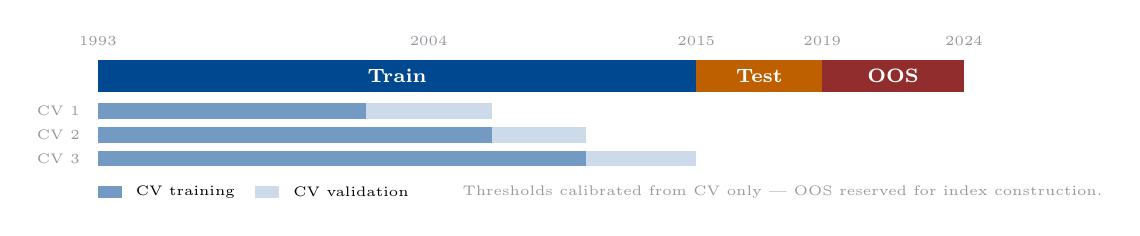
\begin{tikzpicture}[
  font=\scriptsize,
  baseline,
  >=stealth, thick,
]
% --- Year axis -----------------------------------------------------
\foreach \x/\year in {0/1993, 4.2/2004, 7.6/2015, 9.2/2019, 11.0/2024} {
  \node[anchor=south, darkgrey] at (\x,1.55) {\tiny\year};
}

% Main split: train (1993-2015, x=0..7.6), test (2015-2019, x=7.6..9.2), OOS (2019-2024, x=9.2..11.0)
\fill[MainColour]   (0.0,1.10) rectangle (7.6,1.50);
\node[white] at (3.8,1.30) {\textbf{Train}};

\fill[orange!75!black] (7.6,1.10) rectangle (9.2,1.50);
\node[white] at (8.4,1.30) {\textbf{Test}};

\fill[warningRed]   (9.2,1.10) rectangle (11.0,1.50);
\node[white] at (10.1,1.30) {\textbf{OOS}};

% Expanding-window CV bars
\node[anchor=east, darkgrey] at (-0.1,0.85) {\tiny CV 1};
\fill[MainColour!55] (0.0,0.75) rectangle (3.4,0.95);
\fill[MainColour!20] (3.4,0.75) rectangle (5.0,0.95);

\node[anchor=east, darkgrey] at (-0.1,0.55) {\tiny CV 2};
\fill[MainColour!55] (0.0,0.45) rectangle (5.0,0.65);
\fill[MainColour!20] (5.0,0.45) rectangle (6.2,0.65);

\node[anchor=east, darkgrey] at (-0.1,0.25) {\tiny CV 3};
\fill[MainColour!55] (0.0,0.15) rectangle (6.2,0.35);
\fill[MainColour!20] (6.2,0.15) rectangle (7.6,0.35);

% CV legend
\fill[MainColour!55] (0.0,-0.25) rectangle (0.3,-0.10);
\node[anchor=west] at (0.35,-0.175) {\tiny CV training};
\fill[MainColour!20] (2.0,-0.25) rectangle (2.3,-0.10);
\node[anchor=west] at (2.35,-0.175) {\tiny CV validation};
\node[anchor=west, darkgrey] at (4.5,-0.175) {\tiny Thresholds calibrated from CV only --- OOS reserved for index construction.};
\end{tikzpicture}
\end{center}

\vspace{0.4em}

\textbf{Final feature-set keys}

\vspace{0.3em}
\begin{center}
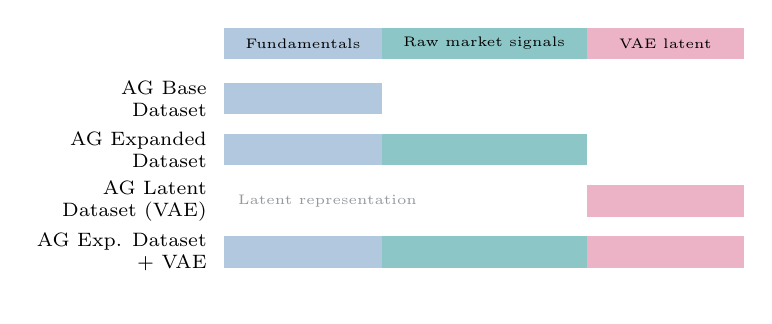
\begin{tikzpicture}[
  font=\scriptsize,
  baseline,
]
% Legend row
\fill[MainColour!30]     (3.0,3.0) rectangle (5.0,3.4); \node at (4.0,3.2){\tiny Fundamentals};
\fill[teal!45]           (5.0,3.0) rectangle (7.6,3.4); \node at (6.3,3.2){\tiny Raw market signals};
\fill[purple!30]         (7.6,3.0) rectangle (9.6,3.4); \node at (8.6,3.2){\tiny VAE latent};

% Row: AG Base Dataset
\node[anchor=east, align=right] at (2.9,2.5){AG Base\\Dataset};
\fill[MainColour!30]     (3.0,2.3) rectangle (5.0,2.7);

% Row: AG Expanded Dataset
\node[anchor=east, align=right] at (2.9,1.85){AG Expanded\\Dataset};
\fill[MainColour!30]     (3.0,1.65) rectangle (5.0,2.05);
\fill[teal!45]           (5.0,1.65) rectangle (7.6,2.05);

% Row: AG Latent Dataset (VAE)
\node[anchor=east, align=right] at (2.9,1.20){AG Latent\\Dataset (VAE)};
\fill[purple!30]         (7.6,1.00) rectangle (9.6,1.40);
\node[anchor=west, darkgrey] at (3.05,1.20){\tiny Latent representation};

% Row: AG Exp. Dataset + VAE
\node[anchor=east, align=right] at (2.9,0.55){AG Exp. Dataset\\+ VAE};
\fill[MainColour!30]     (3.0,0.35) rectangle (5.0,0.75);
\fill[teal!45]           (5.0,0.35) rectangle (7.6,0.75);
\fill[purple!30]         (7.6,0.35) rectangle (9.6,0.75);

\end{tikzpicture}
\end{center}

\end{frame}

%==== 14. Modelling II. =======================================================%

\begin{frame}{Modelling II: Results Temporary CSI}
\scriptsize
\begin{block}{Description}
\scriptsize
Temporary CSI is a rare-event classification problem: only 4.74\% of labelled firm-years are positives. Because of this class imbalance, AP and fixed-FPR recall are more decision-relevant than AUC alone. AG Exp. Dataset + VAE ranks best in CV, while AG Expanded Dataset is strongest on the 2016-2019 test split.
\end{block}

\vspace{0.05em}
\begin{table}[ht]
\centering
\setlength{\tabcolsep}{2.8pt}
\begin{tabular}{L{2.65cm}R{0.85cm}R{0.85cm}R{0.9cm}R{0.9cm}R{0.9cm}R{0.95cm}}
\toprule
Model & CV-AP & CV-AUC & CV-FPR3 & Test-AP & Test-AUC & Test-FPR3 \\
\midrule
AG Expanded Dataset & 0.2046 & 0.8635 & 0.2344 & \textbf{0.1985} & \textbf{0.8766} & \textbf{0.2002} \\
AG Base Dataset & 0.1923 & 0.8446 & 0.2206 & 0.1656 & 0.8538 & 0.1517 \\
AG Latent Dataset (VAE) & 0.1659 & 0.8454 & 0.1706 & 0.1501 & 0.8438 & 0.1294 \\
AG Exp. Dataset + VAE & \textbf{0.2114} & \textbf{0.8667} & \textbf{0.2478} & 0.1864 & 0.8741 & 0.1779 \\
\bottomrule
\end{tabular}
\end{table}

\remarkfoot{CV-FPR3 and Test-FPR3 are R@FPR3. OOS, R@FPR1, R@FPR5, Brier, and full split tables are in Appendix A10.}

\vspace{0.1em}
\begin{alertblock}{Interpretation}
\scriptsize
Test-AP improves from the 4.44\% test prevalence baseline to 19.85\%, showing meaningful concentration of CSI cases near the top of the risk ranking. Test-AUC of 0.8766 confirms strong broad ranking, but AP is the more useful indicator for practical screening.
\end{alertblock}

\end{frame}

%==== 15. Modelling III. ======================================================%

\begin{frame}{Modelling III: Results Permanent-CSI}
\scriptsize
\begin{block}{Description}
\scriptsize
Permanent CSI is the harder task: positives are rarer than temporary CSI, with only 3.34\% positives in the full labelled sample and 3\% in the test split. Despite this, the models still rank risk well. AG Expanded Dataset remains the reporting baseline, while AG Exp. Dataset + VAE is the strongest non-raw challenger on CV/test.
\end{block}

\vspace{0.05em}
\begin{table}[ht]
\centering
\setlength{\tabcolsep}{2.8pt}
\begin{tabular}{L{2.65cm}R{0.85cm}R{0.85cm}R{0.9cm}R{0.9cm}R{0.9cm}R{0.95cm}}
\toprule
Model & CV-AP & CV-AUC & CV-FPR3 & Test-AP & Test-AUC & Test-FPR3 \\
\midrule
AG Expanded Dataset & 0.1854 & \textbf{0.8757} & \textbf{0.2607} & \textbf{0.1416} & 0.8810 & 0.1808 \\
AG Base Dataset & 0.1785 & 0.8677 & 0.2379 & 0.1289 & 0.8627 & 0.1697 \\
AG Latent Dataset (VAE) & 0.1426 & 0.8460 & 0.1960 & 0.1115 & 0.8496 & 0.1513 \\
AG Exp. Dataset + VAE & \textbf{0.1883} & 0.8719 & 0.2578 & 0.1415 & \textbf{0.8838} & \textbf{0.2011} \\
\bottomrule
\end{tabular}
\end{table}

\remarkfoot{CV-FPR3 and Test-FPR3 are R@FPR3. OOS, R@FPR1, R@FPR5, Brier, and full split tables are in Appendix A11.}

\vspace{0.1em}
\begin{alertblock}{Interpretation}
\scriptsize
Temporary CSI has more positives and higher test prevalence: 4.44\% vs 3\%. Permanent CSI is therefore harder and more affected by class imbalance. AUC is similar or slightly higher for permanent CSI, but AP is lower because the base prevalence is lower. AG Expanded Dataset and AG Exp. Dataset + VAE are nearly tied on Test-AP: 0.1416 vs 0.1415. AG Exp. Dataset + VAE has the best Test-AUC and Test-FPR3, so it is a strong challenger, but not a clean replacement for the reporting baseline.
\end{alertblock}

\end{frame}


%==== 16. Modelling Summary. ==================================================%

\begin{frame}{\small Modelling Summary: the Models Rank Implosion Risk Well}
\footnotesize

\begin{center}
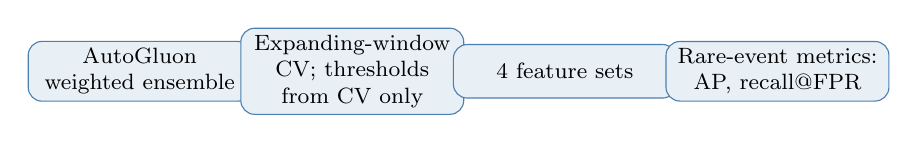
\begin{tikzpicture}[
  font=\footnotesize,
  pill/.style={draw=MainColour!70, fill=MainColour!9, rounded corners=5pt,
    text width=2.62cm, align=center, inner xsep=3pt, inner ysep=2.5pt,
    minimum height=0.68cm}
]
\node[pill] at (-4.05,0) {AutoGluon weighted ensemble};
\node[pill] at (-1.35,0) {Expanding-window CV; thresholds from CV only};
\node[pill] at (1.35,0) {4 feature sets};
\node[pill] at (4.05,0) {Rare-event metrics: AP, recall@FPR};
\end{tikzpicture}
\end{center}

\vspace{-0.1em}
\begin{columns}[T,onlytextwidth]
\begin{column}{0.49\textwidth}
\textbf{Test Average Precision vs random baseline (prevalence)}

\vspace{0.2em}
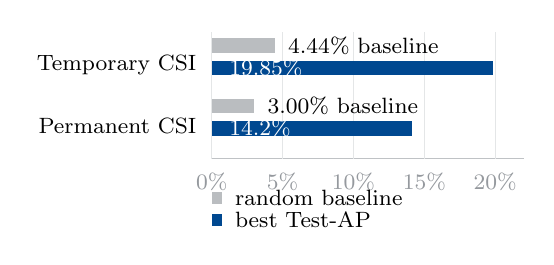
\begin{tikzpicture}[font=\footnotesize, xscale=0.18, yscale=0.85]
  \draw[darkgrey!60] (0,-0.15) -- (22,-0.15);
  \foreach \x in {0,5,10,15,20} {
    \draw[darkgrey!25] (\x,-0.15) -- (\x,1.75);
    \node[anchor=north, darkgrey] at (\x,-0.22) {\x\%};
  }
  \node[anchor=east] at (-0.4,1.25) {Temporary CSI};
  \node[anchor=east] at (-0.4,0.35) {Permanent CSI};

  \fill[darkgrey!65] (0,1.43) rectangle (4.44,1.65);
  \fill[MainColour] (0,1.10) rectangle (19.85,1.32);
  \fill[darkgrey!65] (0,0.53) rectangle (3.00,0.75);
  \fill[MainColour] (0,0.20) rectangle (14.16,0.42);

  \node[anchor=west] at (4.70,1.54) {4.44\% baseline};
  \node[anchor=west] at (0.55,1.21) {\textcolor{white}{19.85\%}};
  \node[anchor=west] at (3.25,0.64) {3.00\% baseline};
  \node[anchor=west] at (0.55,0.31) {\textcolor{white}{14.2\%}};

  \fill[darkgrey!65] (0,-0.82) rectangle (0.75,-0.64);
  \node[anchor=west] at (0.95,-0.73) {random baseline};
  \fill[MainColour] (0,-1.15) rectangle (0.75,-0.97);
  \node[anchor=west] at (0.95,-1.06) {best Test-AP};
\end{tikzpicture}
\end{column}

\begin{column}{0.47\textwidth}
\textbf{\color{MainColour}Result.}
Test-AUC is around $0.88$, recall@FPR3 is around $0.20$, and Test-AP is about $4.5$--$4.7\times$ the base rate.\\[4pt]

\textbf{\color{MainColour}Verdict.}
\agexp{} is the reporting baseline; \agvae{} is the strongest challenger. Weighted ensembles top the leaderboards, and tree families carry the useful signal.\\[4pt]

\textbf{\color{MainColour}Subquestions.}
VAE augments rather than replaces the expanded feature set; feature drivers move to the appendix.
\end{column}
\end{columns}

\vspace{0.35em}
\begin{block}{Hand-off}
\footnotesize
Calibrated scores become exclusion signals for the index; the question shifts from ``can we rank risk?'' to ``does removing flagged firms improve the index?''
\end{block}
\remarkfoot{Model metrics and caveats are in Appendix A10--A13.}
\end{frame}

%==== 17. False-positive bridge. =============================================%

% Generated for AE-SLIDE-CLEANUP-002 from saved prediction artifacts.
% CV source: 03_Data_Output/6_ModelSuite/raw/temporary_csi/ag_cv_results.parquet
% Test source: 03_Data_Output/6_ModelSuite/raw/temporary_csi/ag_preds_test_eval.parquet
\newcommand{\slideSeventeenTau}{0.217}
\newcommand{\slideSeventeenTestFpr}{8.7\%}
\newcommand{\slideSeventeenTestRecall}{45.9\%}
\newcommand{\slideSeventeenTpCount}{369}
\newcommand{\slideSeventeenFpCount}{1,502}
\newcommand{\slideSeventeenAdjacentShare}{10.8\%}
\newcommand{\slideSeventeenOverlapShare}{100.0\%}


\begin{frame}{Why the Screen Cannot Be Perfect}
\scriptsize
\textbf{Temporary CSI, \agexp{}:} FPR3 threshold calibrated on CV predictions only, then applied to the 2016--2019 test set.

\vspace{0.15em}
\begin{columns}[T,onlytextwidth]
\begin{column}{0.54\textwidth}
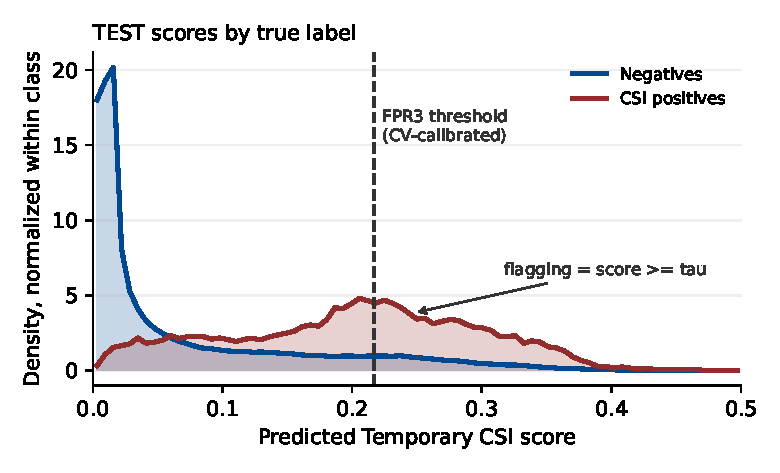
\includegraphics[width=\linewidth]{slide17_fp_bridge_density.pdf}
\end{column}

\begin{column}{0.43\textwidth}
\textbf{\color{MainColour}Live test diagnostic}
\begin{itemize}
  \setlength\itemsep{0.15em}
  \item CV-calibrated $\tau=\slideSeventeenTau$; test FPR is \slideSeventeenTestFpr{} and recall is \slideSeventeenTestRecall{}.
  \item The rule flags \slideSeventeenTpCount{} true CSI rows and \slideSeventeenFpCount{} negatives in test.
  \item Only \slideSeventeenAdjacentShare{} of false positives are threshold-adjacent.
  \item \slideSeventeenOverlapShare{} of false positives overlap the flagged true-positive score range.
\end{itemize}
Raising the threshold would remove some false positives, but it would also drop real CSI firms.
\end{column}
\end{columns}

\vspace{0.05em}
\begin{alertblock}{What this means for the index}
\scriptsize
The screen is useful but structurally imperfect. CSI firms are a small cap-weighted exposure, so false positives and retained-stock reweighting create a dilution ceiling. This is not simply a model failure; it frames the attribution slide.
\end{alertblock}
\vspace{-0.2em}
\remarkfoot{Threshold is CV-calibrated; distribution and counts use the 2016--2019 test set; \agexp{}; temporary CSI. Threshold-adjacent means a false-positive score in $[\tau,\tau+0.01]$, matching the prior false-positive diagnostic.}
\end{frame}

%==== 18. VAE modelling nuance. =============================================%

\begin{frame}{Modelling V: VAE Features --- Benefits and Drawbacks}
\scriptsize
\textbf{Autoencoder/AP subquestion.} How does the integration of Autoencoders for feature engineering impact the Average Precision of Ensemble models compared to those trained solely on raw financial data?

\vspace{0.25em}
\begin{columns}[T,onlytextwidth]
\begin{column}{0.49\textwidth}
\begin{block}{Benefits}
\scriptsize
\begin{itemize}
  \setlength\itemsep{0.22em}
  \item Among VAE/non-raw variants, \agvae{} leads CV-AP in both tracks: temporary $0.2114$, permanent $0.1883$.
  \item Temporary OOS: \agvae{} leads AP $0.3152$; R@FPR1/3/5 is $0.1051$ / $0.2632$ / $0.4128$.
  \item Permanent test: \agvae{} leads AUC $0.8838$ and FPR3/5 recall $0.2011$ / $0.3155$.
  \item Permanent OOS: \aglatent{} leads AP/AUC/Brier/FPR recall: AP $0.0482$, AUC $0.8337$.
\end{itemize}
\end{block}
\end{column}

\begin{column}{0.49\textwidth}
\begin{block}{Drawbacks}
\scriptsize
\begin{itemize}
  \setlength\itemsep{0.22em}
  \item VAE does not replace expanded-data information.
  \item \agexp{} keeps slightly higher temporary OOS AUC: $0.8961$ vs.\ $0.8950$.
  \item \agexp{} is the cleaner reporting baseline.
  \item Latent-only is weaker on temporary CV/test and mainly competitive for permanent OOS.
  \item Added architecture and compute cost.
\end{itemize}
\end{block}
\end{column}
\end{columns}

\vspace{0.25em}
\begin{alertblock}{Verdict}
\scriptsize
Autoencoder features improve Average Precision as an augmentation, especially when combined with expanded features, but do not dominate AUC and do not replace raw/fundamental information.
\end{alertblock}

\remarkfoot{Values use current model-suite threshold metrics: \texttt{03\_Data\_Output/6\_ModelSuite/derived\_metrics/complete\_threshold\_metrics\_wide.csv}; raw comparator metrics use \texttt{raw/metric\_snapshot.csv}.}
\end{frame}

%==== 19. Index Construction E. ===============================================%

\section{E. Index Construction}
\begin{frame}{Index Construction I: From Score to Portfolio Weight}
\small

\begin{alertblock}{One score rule, two exclusion regimes}
\scriptsize
The model produces a probability of CSI next year. A threshold turns that probability into a binary exclusion flag. The flag is then applied to market-cap weights. Two regimes differ only in how long the flag persists after it first fires.
\end{alertblock}

\vspace{0.5em}

\textbf{From model score to portfolio weight}

\vspace{0.3em}
\begin{center}
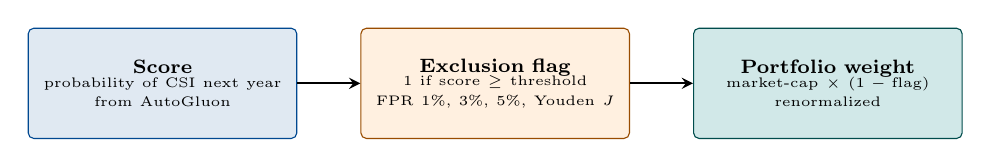
\begin{tikzpicture}[
  font=\scriptsize,
  pipebox/.style={draw, rounded corners=2pt, minimum height=14mm, text width=3.2cm, align=center, inner sep=3pt},
  scorebox/.style={pipebox, fill=MainColour!12, draw=MainColour},
  flagbox/.style={pipebox, fill=orange!12, draw=orange!60!black},
  weightbox/.style={pipebox, fill=teal!18, draw=teal!60!black},
  pipearrow/.style={->, >=stealth, thick}
]
\node[scorebox] (score) {\textbf{Score}\\[-1pt]\tiny probability of CSI next year\\[-1pt]\tiny from AutoGluon};
\node[flagbox, right=8mm of score] (flag) {\textbf{Exclusion flag}\\[-1pt]\tiny 1 if score $\geq$ threshold\\[-1pt]\tiny FPR 1\%, 3\%, 5\%, Youden $J$};
\node[weightbox, right=8mm of flag] (weight) {\textbf{Portfolio weight}\\[-1pt]\tiny market-cap $\times$ $(1-\text{flag})$\\[-1pt]\tiny renormalized};
\draw[pipearrow] (score) -- (flag);
\draw[pipearrow] (flag) -- (weight);
\end{tikzpicture}
\end{center}

\vspace{0.5em}

\textbf{How the flag evolves over time} {\scriptsize\color{darkgrey} --- a firm crosses the threshold in year 3}

\vspace{0.3em}
\begin{center}
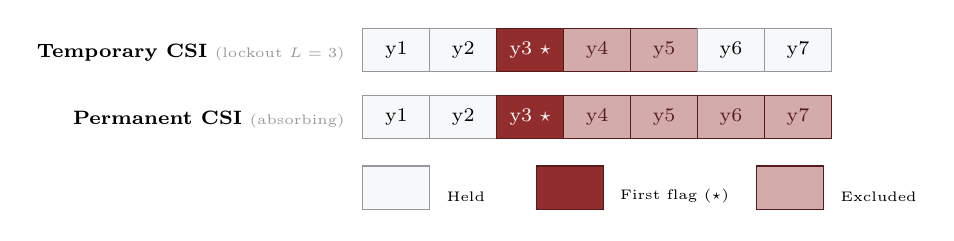
\begin{tikzpicture}[
  font=\scriptsize,
  cell/.style={draw, minimum width=0.85cm, minimum height=0.55cm, inner sep=0pt, anchor=south west},
  held/.style={cell, fill=grey!20, draw=darkgrey},
  flag/.style={cell, fill=warningRed, draw=warningRed!60!black, text=white},
  excl/.style={cell, fill=warningRed!40, draw=warningRed!60!black, text=warningRed!60!black}
]
\node[anchor=east] at (-0.1,1.05) {\scriptsize\textbf{Temporary CSI} \tiny\color{darkgrey}(lockout $L=3$)};
\foreach \i in {0,1} \node[held] at (\i*0.85,0.8) {y\the\numexpr\i+1\relax};
\node[flag] at (1.7,0.8) {y3 $\star$};
\foreach \i in {0,1} \node[excl] at (2.55+\i*0.85,0.8) {y\the\numexpr\i+4\relax};
\foreach \i in {0,1} \node[held] at (4.25+\i*0.85,0.8) {y\the\numexpr\i+6\relax};

\node[anchor=east] at (-0.1,0.20) {\scriptsize\textbf{Permanent CSI} \tiny\color{darkgrey}(absorbing)};
\foreach \i in {0,1} \node[held] at (\i*0.85,-0.05) {y\the\numexpr\i+1\relax};
\node[flag] at (1.7,-0.05) {y3 $\star$};
\foreach \i in {0,...,3} \node[excl] at (2.55+\i*0.85,-0.05) {y\the\numexpr\i+4\relax};

\node[held, anchor=south west] at (0.0,-0.95) {};
\node[anchor=west] at (0.95,-0.78) {\tiny Held};
\node[flag, anchor=south west] at (2.2,-0.95) {};
\node[anchor=west] at (3.15,-0.78) {\tiny First flag ($\star$)};
\node[excl, anchor=south west] at (5.0,-0.95) {};
\node[anchor=west] at (5.95,-0.78) {\tiny Excluded};
\end{tikzpicture}
\end{center}

\end{frame}

%==== 18. Index Construction I ================================================%

\begin{frame}{Index Construction II: Universes and Comparators}
\small

\begin{alertblock}{Same exclusion rule, four universes}
\scriptsize
The calibrated score-to-weight pipeline is applied independently inside each universe, so each screened index is evaluated against the matching unfiltered benchmark.
\end{alertblock}

\vspace{0.45em}

\begin{center}
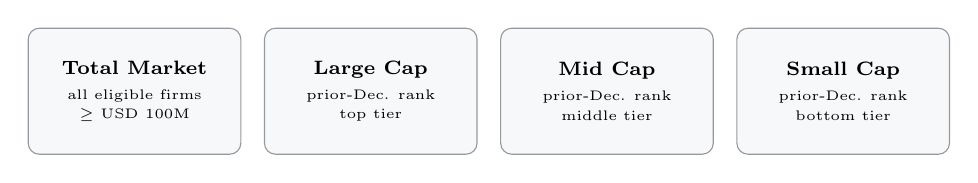
\begin{tikzpicture}[
  font=\scriptsize,
  uni/.style={draw=darkgrey, fill=grey!20, rounded corners=4pt, minimum width=2.7cm, minimum height=1.6cm, align=center}
]
\node[uni] (tm) at (0,0)   {\textbf{Total Market}\\[1pt]\tiny all eligible firms\\[-1pt]\tiny $\geq$ USD 100M};
\node[uni] (lc) at (3.0,0) {\textbf{Large Cap}\\[1pt]\tiny prior-Dec. rank\\[-1pt]\tiny top tier};
\node[uni] (mc) at (6.0,0) {\textbf{Mid Cap}\\[1pt]\tiny prior-Dec. rank\\[-1pt]\tiny middle tier};
\node[uni] (sc) at (9.0,0) {\textbf{Small Cap}\\[1pt]\tiny prior-Dec. rank\\[-1pt]\tiny bottom tier};
\end{tikzpicture}
\end{center}

\vspace{0.15em}
\begin{center}
\scriptsize\textit{Tier breakpoints: \textless{}author to insert exact Large/Mid/Small cap thresholds\textgreater{}}
\end{center}

\vspace{0.25em}

\begin{columns}[t]
\begin{column}{0.49\textwidth}
\textbf{Universe construction}
\scriptsize
\begin{itemize}
  \item Total Market keeps all eligible firms above USD 100 million market cap.
  \item Large, Mid, and Small Cap are formed by prior-December market-cap rank.
  \item Quarterly rebalancing: March, June, September, December.
  \item Within each universe, portfolio weights start from market capitalization.
\end{itemize}
\end{column}
\begin{column}{0.49\textwidth}
\textbf{Comparators}
\scriptsize
\begin{itemize}
  \item Primary comparator: the unfiltered cap-weighted benchmark in the same universe.
  \item Screened portfolios are therefore compared like-for-like: Total vs Total, Large vs Large, Mid vs Mid, Small vs Small.
  \item Min-volatility and quality screens are planned extensions under the main research question; see limitations.
\end{itemize}
\end{column}
\end{columns}

\end{frame}

%==== 20. Headline / Verdict (NEW) ===========================================%
\begin{frame}{Index Results: Does the Crash Filter Help?}
\small

\vspace{0.3em}

\begin{columns}[T]
\begin{column}{0.55\textwidth}
\centering
{\scriptsize Benchmark-relative alpha by universe (pp, 10 bps net)}\\[3pt]

\begin{tikzpicture}[font=\tiny, yscale=0.9]
  \fill[MainColour]  (0,0)   rectangle (0.22,0.22);
  \node[anchor=west] at (0.28,0.11) {OOS 2020--24};
  \fill[posgreenL]   (2.45,0) rectangle (2.67,0.22);
  \node[anchor=west] at (2.73,0.11) {Test 2016--19};
\end{tikzpicture}\\[2pt]
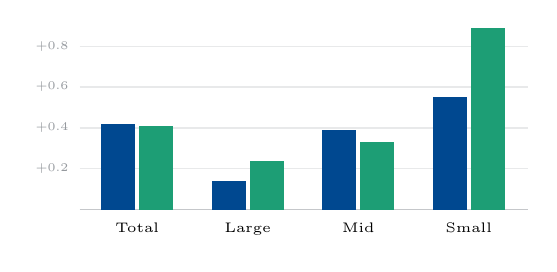
\begin{tikzpicture}[font=\tiny, yscale=2.6, xscale=0.78]
  \draw[darkgrey!55] (0,0) -- (7.3,0);
  \foreach \y in {0.2,0.4,0.6,0.8} {
    \draw[darkgrey!22] (0,\y) -- (7.3,\y);
    \node[anchor=east, darkgrey, scale=0.85] at (-0.05,\y) {+\y};
  }
  \foreach \x/\o/\t/\lbl in {0.35/0.42/0.41/Total, 2.15/0.14/0.24/Large,
                             3.95/0.39/0.33/Mid, 5.75/0.55/0.89/Small} {
    \fill[MainColour] (\x,0)      rectangle (\x+0.55,\o);
    \fill[posgreenL]  (\x+0.62,0) rectangle (\x+1.17,\t);
    \node[anchor=north, black] at (\x+0.585,-0.015) {\lbl};
  }
\end{tikzpicture}
\end{column}
\begin{column}{0.43\textwidth}
\scriptsize
\textbf{\color{MainColour}OOS alpha.} Current OOS deltas are positive in all four universes; Mid and Small are strongest.\\[5pt]
\textbf{\color{MainColour}Test-set check.} Test evidence is shown separately; Permanent-CSI Total Sharpe rises $0.89 \to \mathbf{1.00}$.\\[5pt]
\textbf{\color{MainColour}Source of alpha.} Mostly retained-name reweighting, not direct event-avoidance (next slides).
\end{column}
\end{columns}

\begin{alertblock}{Summary}
\scriptsize
The crash-filter appears beneficial in both evaluation windows, but the evidence differs by split. The OOS result is a positive benchmark-relative return delta across the four universes. The test-set result is reported separately and should not be read as the same diagnostic as OOS risk performance.
\end{alertblock}

\end{frame}

%==== 21. Temporary-CSI Results ==========================================%
\begin{frame}{Temporary-CSI Results: OOS (2020-2024) with 10 bps of Transaction Costs}
\scriptsize
\textbf{Best strategy per universe net of 10 bps costs vs.\ the zero-cost market-weighted benchmark.}
\vspace{0.3em}

\begin{table}[ht]
\centering
\setlength{\tabcolsep}{4pt}
\renewcommand{\arraystretch}{1.25}
\begin{tabular}{L{0.95cm}L{3.1cm}R{1.7cm}R{0.8cm}@{\hspace{1.8em}}R{1.7cm}R{1.9cm}}
\toprule
 & & \multicolumn{2}{c}{\textbf{Return}} & \multicolumn{2}{c}{\textbf{\color{MainColour}Risk}} \\
\cmidrule(lr){3-4}\cmidrule(lr){5-6}
Universe & Strategy & Geo ret. & $\Delta$ pp & Sharpe & Max DD \\
\midrule
Total & \agbase; Youden 3y & $13.3 \to 13.7$ & $+0.42$ & $0.60 \to \mathbf{0.64}$ & $-25.0 \to \mathbf{-23.8}$ \\
Large & \agbase; Youden 3y & $14.3 \to 14.4$ & $+0.14$ & $0.66 \to \mathbf{0.68}$ & $-24.8 \to \mathbf{-23.9}$ \\
Mid   & \agbase; FPR5 5y   & $9.7  \to 10.0$ & $+0.39$ & $0.41 \to \mathbf{0.42}$ & $-24.6 \to \mathbf{-24.5}$ \\
Small & \agvae; Youden 3y  & $7.7  \to 8.2$  & \textcolor{posgreen}{$\mathbf{+0.55}$} & $0.31 \to \mathbf{0.33}$ & $-29.1 \to -29.3$ \\
\bottomrule
\end{tabular}
\end{table}

\vspace{0.1em}
\begin{block}{Main takeaway}
\scriptsize
The risk-filter works better the smaller the market cap.: the alpha rises from $+0.14$pp (Large) to $+0.39$pp (Mid) to $+0.55$pp (Small). Smaller-cap universes include more firms in distress and exclusions move a larger part of the portfolio (about 85-106\% turnover vs.\ 10-13\% for the total market). Drawdown improves everywhere except for small caps.
\end{block}
\end{frame}

%==== 22. Permanent-CSI OOS Results ==========================================%
\begin{frame}{Permanent-CSI Results: OOS (2020-2024) with 10 bps of Transaction Costs}
\scriptsize
\textbf{Best strategy per universe net of 10 bps costs vs.\ the zero-cost market-weighted benchmark.}
\vspace{0.3em}

\begin{table}[ht]
\centering
\setlength{\tabcolsep}{4pt}
\renewcommand{\arraystretch}{1.25}
\begin{tabular}{L{0.95cm}L{3.1cm}R{1.7cm}R{0.8cm}@{\hspace{1.8em}}R{1.7cm}R{1.9cm}}
\toprule
 & & \multicolumn{2}{c}{\textbf{Return}} & \multicolumn{2}{c}{\textbf{\color{MainColour}Risk}} \\
\cmidrule(lr){3-4}\cmidrule(lr){5-6}
Universe & Strategy & Geo ret. & $\Delta$ pp & Sharpe & Max DD \\
\midrule
Total & \agvae; FPR5    & $13.3 \to 13.5$ & $+0.26$ & $0.60 \to \mathbf{0.61}$ & $-25.0 \to \mathbf{-24.7}$ \\
Large & \agvae; FPR5    & $14.3 \to 14.5$ & $+0.22$ & $0.66 \to \mathbf{0.67}$ & $-24.8 \to \mathbf{-24.5}$ \\
Mid   & \agbase; FPR5   & $9.7  \to 10.3$ & \textcolor{posgreen}{$\mathbf{+0.62}$} & $0.41 \to \mathbf{0.44}$ & $-24.6 \to \mathbf{-24.5}$ \\
Small & \aglatent; FPR3 & $7.7  \to 7.9$  & $+0.24$ & $0.31 \to \mathbf{0.32}$ & $-29.1 \to -29.3$ \\
\bottomrule
\end{tabular}
\end{table}

\vspace{0.1em}
\begin{block}{Main takeaway}
\scriptsize
The permanent filter tilts the gains toward Mid Cap ($+0.62$pp), its strongest universe. Direction matches the temporary track, but more exclusion over-removes firms with broad thresholds, which is why Youden is dropped in favour of FPR3 and FPR5.
\end{block}
\end{frame}

%==== 23. Attribution: Where Does the Alpha Come From? =======================%
\begin{frame}{Where Does the Alpha Come From?}
\scriptsize

\begin{alertblock}{It is not direct event-avoidance}
\scriptsize
Because positives are rare, realized alpha is dominated by reweighting retained firms, not by directly dodging CSI events. A large false-positive opportunity cost is the main offset. For this reason, most of the performance gain disappears.
\end{alertblock}

\vspace{0.2em}
{\scriptsize Decomposition for Total Market, OOS (pp): TP $+$ FP $+$ reweight $+$ cost $+$ geo $=$ alpha}\\[2pt]
\begin{center}
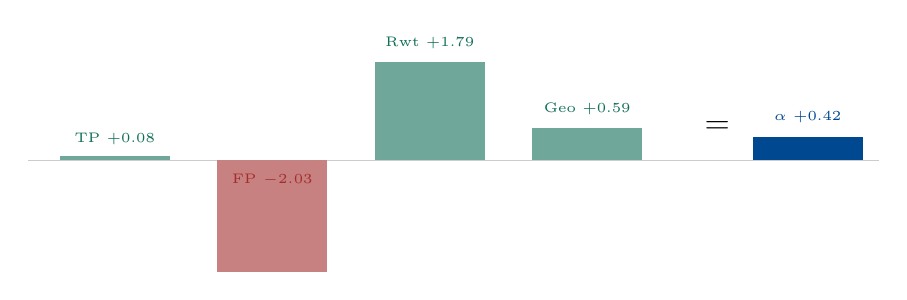
\begin{tikzpicture}[font=\tiny, yscale=0.7]
  \draw[darkgrey!50] (-0.2,0) -- (10.6,0);
  % value, x-left, colour, label
  \foreach \v/\x/\c/\lbl in {0.08/0.2/posgreen/{TP +0.08}, -2.03/2.2/negred/{FP $-2.03$},
                             1.79/4.2/posgreen/{Rwt +1.79}, 0.59/6.2/posgreen/{Geo +0.59}} {
    \fill[\c!60] (\x,0) rectangle (\x+1.4,\v);
  }
  \node[anchor=south, posgreen] at (0.9,0.1)  {TP +0.08};
  \node[anchor=north, negred]   at (2.9,-0.08){FP $-2.03$};
  \node[anchor=south, posgreen] at (4.9,1.85) {Rwt +1.79};
  \node[anchor=south, posgreen] at (6.9,0.65) {Geo +0.59};
  \node at (8.55,0.6) {\large $=$};
  \fill[MainColour] (9.0,0) rectangle (10.4,0.42);
  \node[anchor=south, MainColour] at (9.7,0.5) {$\alpha$ +0.42};
\end{tikzpicture}
\end{center}

\vspace{0.2em}
\begin{table}[ht]
\centering
\setlength{\tabcolsep}{5pt}\renewcommand{\arraystretch}{1.15}
\begin{tabular}{L{3.0cm}R{1.0cm}R{1.0cm}R{1.4cm}R{1.0cm}R{1.0cm}R{1.1cm}}
\toprule
Universe (OOS, temp) & TP & FP & Reweight & TC & Geo & Alpha \\
\midrule
Total & $+0.08$ & \textcolor{negred}{$-2.03$} & \textcolor{posgreen}{$+1.79$} & $-0.01$ & $+0.59$ & $\mathbf{+0.42}$ \\
Large & $+0.00$ & \textcolor{negred}{$-1.50$} & \textcolor{posgreen}{$+1.24$} & $-0.01$ & $+0.41$ & $\mathbf{+0.14}$ \\
Mid   & $-0.00$ & $+0.05$ & \textcolor{posgreen}{$+0.27$} & $-0.11$ & $+0.18$ & $\mathbf{+0.39}$ \\
Small & \textcolor{posgreen}{$+0.42$} & \textcolor{negred}{$-4.00$} & \textcolor{posgreen}{$+3.94$} & $-0.09$ & $+0.28$ & $\mathbf{+0.55}$ \\
\bottomrule
\end{tabular}
\end{table}
\end{frame}

%==== 24. Test-Set Validation ================================================%
% TODO: this shows the PERMANENT-Youden test winners (one consistent strategy,
% Total Sharpe crosses 1.0). To show the Temporary winners instead, replace the
% four rows with your temp test winners and the strategy column accordingly.
\begin{frame}{Permanent-CSI Results: Test (2016-2019) with 10 bps of Transaction Costs}
\scriptsize

\begin{table}[ht]
\centering
\setlength{\tabcolsep}{4pt}
\renewcommand{\arraystretch}{1.25}
\begin{tabular}{L{0.95cm}L{3.1cm}R{1.7cm}R{0.8cm}@{\hspace{1.8em}}R{1.7cm}R{1.9cm}}
\toprule
 & & \multicolumn{2}{c}{\textbf{Return}} & \multicolumn{2}{c}{\textbf{\color{MainColour}Risk}} \\
\cmidrule(lr){3-4}\cmidrule(lr){5-6}
Universe & Strategy & Geo ret. & $\Delta$ pp & Sharpe & Max DD \\
\midrule
Total & \agvae; Youden & $13.8 \to 14.2$ & $+0.45$ & $0.89 \to \textcolor{posgreen}{\mathbf{1.00}}$ & $-14.6 \to \mathbf{-12.8}$ \\
Large & \agvae; Youden & $14.2 \to 14.4$ & $+0.26$ & $0.95 \to \textcolor{posgreen}{\mathbf{1.04}}$ & $-13.8 \to \mathbf{-12.2}$ \\
Mid   & \agvae; Youden & $13.7 \to 14.2$ & $+0.43$ & $0.84 \to \mathbf{0.95}$ & $-15.3 \to \mathbf{-13.8}$ \\
Small & \agvae; Youden & $11.4 \to 12.2$ & \textcolor{posgreen}{$\mathbf{+0.83}$} & $0.58 \to \mathbf{0.68}$ & $-20.1 \to \mathbf{-18.3}$ \\
\bottomrule
\end{tabular}
\end{table}

\vspace{0.1em}
\begin{block}{Validation Summary}
\scriptsize
In the calmer 2016-2019 window a single consistent strategy (Exp. Dataset + VAE with Youden computed thresholds) improves Sharpe and cuts drawdown in every universe, with Total Sharpe crossing 1.0. The same small-cap tilt appears ($+0.83$pp Small vs.\ $+0.26$pp Large).
\end{block}
\end{frame}

%==== 28. Transaction-Cost Robustness ========================================%
\begin{frame}{Impact of transaction costs: the winners are unchanged}
\scriptsize
\textbf{Selected OOS winners when assuming transaction costs of 5, 10 and 20 bps.}
\vspace{0.3em}

\begin{table}[ht]
\centering
\setlength{\tabcolsep}{4pt}\renewcommand{\arraystretch}{1.2}
\begin{tabular}{L{0.95cm}L{0.95cm}L{2.9cm}R{2.7cm}R{1.6cm}}
\toprule
Track & Universe & Selected OOS winner & Active $\alpha$ (5/10/20) & Ranking \\
\midrule
Temp. & Total & \agbase; Youden 3y & $+0.43 / +0.42 / +0.41$ & \textcolor{posgreen}{unchanged} \\
Temp. & Large & \agbase; Youden 3y & $+0.15 / +0.14 / +0.12$ & \textcolor{posgreen}{unchanged} \\
Temp. & Mid   & \agbase; FPR5 5y   & $+0.45 / +0.39 / +0.28$ & \textcolor{posgreen}{unchanged} \\
Temp. & Small & \agvae; Youden 3y  & $+0.59 / +0.55 / +0.45$ & \textcolor{posgreen}{unchanged} \\
Perm. & Total & \agvae; FPR5       & $+0.26 / +0.26 / +0.25$ & \textcolor{posgreen}{unchanged} \\
Perm. & Large & \agvae; FPR5       & $+0.22 / +0.22 / +0.20$ & \textcolor{posgreen}{unchanged} \\
Perm. & Mid   & \agbase; FPR5      & $+0.68 / +0.62 / +0.51$ & \textcolor{posgreen}{unchanged} \\
Perm. & Small & \aglatent; FPR3    & $+0.28 / +0.24 / +0.16$ & \textcolor{posgreen}{unchanged} \\
\bottomrule
\end{tabular}
\end{table}

\vspace{0.1em}
\begin{block}{Takeaway}
\scriptsize
Raising costs to 20 bps lowers net returns but does not change a single winner or flip the strategy ranking.
\end{block}
\remarkfoot{Active alpha is measured versus the zero-cost market-cap benchmark; only the strategy pays transaction costs.}
\end{frame}

%==== 29. Turnover Effect (table -> chart) ===================================%
\begin{frame}{Cost Drag due to turnover is concentrated in mid and small caps}
\scriptsize
{\scriptsize Annualized gross buy $+$ sell turnover of the selected OOS strategies (\%)}\\[3pt]
\begin{center}

\begin{tikzpicture}[font=\tiny]
  \fill[MainColour] (0,0) rectangle (0.22,0.22);
  \node[anchor=west] at (0.28,0.11) {Temporary};
  \fill[posgreenL]  (2.2,0) rectangle (2.42,0.22);
  \node[anchor=west] at (2.48,0.11) {Permanent};
\end{tikzpicture}\\[2pt]
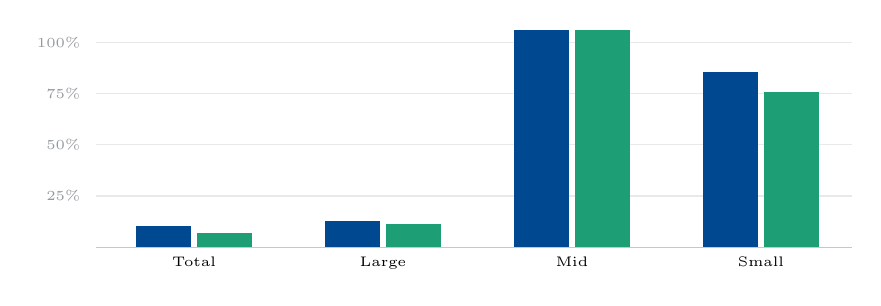
\begin{tikzpicture}[font=\tiny, yscale=0.026, xscale=1.0]
  \draw[darkgrey!55] (0,0) -- (9.6,0);
  \foreach \y in {25,50,75,100} {
    \draw[darkgrey!22] (0,\y) -- (9.6,\y);
    \node[anchor=east, darkgrey] at (-0.08,\y) {\y\%};
  }
  \foreach \x/\tmp/\prm/\lbl in {0.5/10.4/6.8/Total, 2.9/13.0/11.5/Large,
                                 5.3/105.9/106.2/Mid, 7.7/85.5/75.7/Small} {
    \fill[MainColour] (\x,0)      rectangle (\x+0.7,\tmp);
    \fill[posgreenL]  (\x+0.78,0) rectangle (\x+1.48,\prm);
    \node[anchor=north, black] at (\x+0.74,0) {\lbl};
  }
\end{tikzpicture}
\end{center}

\vspace{0.1em}
\begin{block}{Summary}
\scriptsize
Drag scales linearly with turnover $\times$ cost. Total and Large are barely traded (between 7-13\%), so their 20 bps drag is at most $0.13$pp. Mid and Small rebalancing is comparably larger at 75-106\% a year, lifting their 20 bps drag to roughly $0.76$-$1.06$pp. Yet, the winner ranking on the previous slide still holds.
\end{block}

\end{frame}

%==== 30. Threshold Families (two tables -> two cards) =======================%
\begin{frame}{The Selected Rules Are Principled, Not Grid-Mined}
\scriptsize

\begin{columns}[T]
\begin{column}{0.48\textwidth}
\begin{block}{Temporary CSI --- finite lockout}
\scriptsize
Youden 3yr wins Total, Large, and Small; FPR5 5yr wins Mid. A recoverable 3--5yr lockout lets the signal age out, capping turnover outside Mid / Small.\\[3pt]
\textbf{20 bps evidence:} Youden has the strongest mean best alpha, $+0.24$pp.
\end{block}
\end{column}
\begin{column}{0.48\textwidth}
\begin{block}{Permanent CSI --- strict FPR}
\scriptsize
FPR5 wins Total, Large, and Mid; FPR3 wins Small. Absorbing removal needs narrower gates --- broad Youden over-removes names and compounds turnover.\\[3pt]
\textbf{20 bps evidence:} FPR3 / FPR5 lead ($+0.24$ / $+0.22$pp); Youden averages $-0.31$pp.
\end{block}
\end{column}
\end{columns}

\vspace{0.4em}
\begin{alertblock}{Why this matters}
\scriptsize
The two tracks select different rule families for a structural reason, not by grid-mining: a temporary flag can expire, so it tolerates a looser cutoff; a permanent flag is irreversible, so cost and turnover mistakes must be gated more tightly. Turnover detail is on the previous slide.
\end{alertblock}
\remarkfoot{Source: \texttt{threshold\_family\_summary\_20bps.csv}; \texttt{best\_by\_track\_index\_cost.csv}.}
\end{frame}

%==== 31. Sensitivity: Main Run vs C/M/T Grid ================================%
% Option: keep your chart1_sensitivity_stability_distribution.png on the left
% via \includegraphics; this TikZ range plot is a reproducible replacement.
\begin{frame}{Sensitivity Analysis: temporary CSI only}
\scriptsize
{\scriptsize Main run versus 24 completed temporary-CSI C/M/T sensitivity runs; relative geometric-return delta (pp).}\\[2pt]
\begin{center}
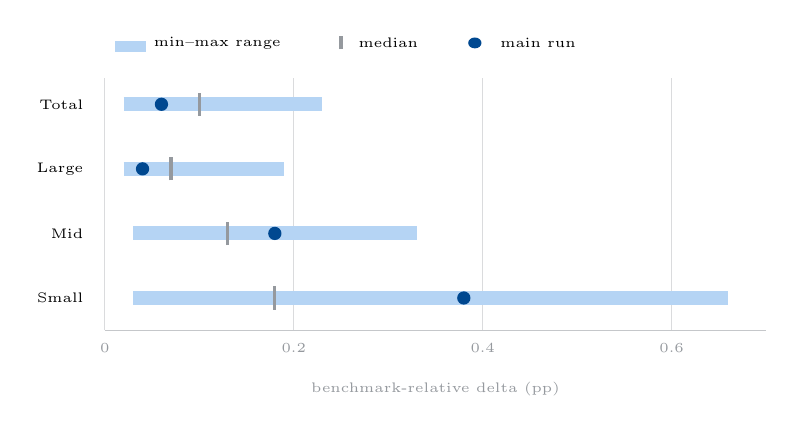
\begin{tikzpicture}[font=\tiny, yscale=0.82]
  % legend
  \node[anchor=west] at (0,3.9) {\tikz\fill[lightblue](0,0)rectangle(0.4,0.14);};
  \node[anchor=west] at (0.5,3.95) {min--max range};
  \draw[darkgrey, line width=1.2pt] (3.0,3.85)--(3.0,4.05);
  \node[anchor=west] at (3.1,3.95) {median};
  \fill[MainColour] (4.7,3.95) circle (2.4pt);
  \node[anchor=west] at (4.9,3.95) {main run};

  % axis frame (x: 0..0.7 pp, scaled by 12)
  \begin{scope}[xscale=12]
    \draw[darkgrey!55] (0,-0.5) -- (0.7,-0.5);
    \foreach \x in {0,0.2,0.4,0.6} {
      \draw[darkgrey!35] (\x,-0.5) -- (\x,3.4);
      \node[anchor=north, darkgrey, scale=1] at (\x,-0.55) {\x};
    }
    % rows: y, min, max, median, main, label
    \foreach \y/\mn/\mx/\md/\mr/\lbl in {3/0.02/0.23/0.10/0.06/Total,
                                         2/0.02/0.19/0.07/0.04/Large,
                                         1/0.03/0.33/0.13/0.18/Mid,
                                         0/0.03/0.66/0.18/0.38/Small} {
      \draw[lightblue, line width=5pt] (\mn,\y) -- (\mx,\y);
      \draw[darkgrey, line width=1.2pt] (\md,\y-0.18) -- (\md,\y+0.18);
      \node[circle, fill=MainColour, inner sep=0pt, minimum size=4.8pt] at (\mr,\y) {};
    }
  \end{scope}
  % row labels (outside xscale so they sit left of the axis)
  \foreach \y/\lbl in {3/Total, 2/Large, 1/Mid, 0/Small}
    \node[anchor=east, black] at (-0.15,\y) {\lbl};
  \node[anchor=north, darkgrey] at (4.2,-1.15) {benchmark-relative delta (pp)};
\end{tikzpicture}
\end{center}

\vspace{-0.8em}
\begin{alertblock}{Robustness read}
\scriptsize
All completed temporary-CSI C/M/T runs stay positive; sensitivity changes magnitude, not sign. Main run: below median in Total/Large, above in Mid/Small. Temporary-CSI evidence only.

\end{alertblock}
\remarkfoot{Temporary CSI only; three blocked-partial configs excluded. Source: \texttt{universe\_stability\_summary.csv}.}
\end{frame}


%==== APPENDIX ================================================================%

\appendix
\section{Appendix}

\begin{frame}{Appendix A1: Dataset, Labels, and Detection Checks}
\scriptsize
\begin{columns}[T,onlytextwidth]
\begin{column}{0.49\textwidth}
\textbf{Failure-label audit}
\vspace{0.15em}
\begin{table}[ht]
\centering
\setlength{\tabcolsep}{2.2pt}
\begin{tabular}{L{2.75cm}R{1.0cm}R{0.95cm}R{1.0cm}}
\toprule
Signal & Firms & Detected & Rate \\
\midrule
CRSP 572--574 & 629 & 545 & 86.65\% \\
CRSP 574 only & 548 & 513 & 93.61\% \\
Adverse 400--490, 550--585 & 5,654 & 3,676 & 65.02\% \\
\bottomrule
\end{tabular}
\end{table}
\vspace{0.25em}
Temporary CSI has 8,517 positive rows and 8,674 unresolved rows. Permanent CSI has 6,258 positive rows and 834 unresolved rows.
\end{column}
\begin{column}{0.49\textwidth}
\textbf{Clean labelled prevalence}
\vspace{0.15em}
\begin{table}[ht]
\centering
\setlength{\tabcolsep}{2.0pt}
\begin{tabular}{L{1.35cm}L{0.8cm}R{0.85cm}R{0.75cm}R{0.75cm}}
\toprule
Track & Split & Labelled & Pos. & Prev. \\
\midrule
Temp. & Train & 143,173 & 6,543 & 4.57\% \\
Temp. & Test & 18,111 & 804 & 4.44\% \\
Temp. & OOS & 18,502 & 1,170 & 6.32\% \\
Perm. & Train & 143,173 & 5,379 & 3.76\% \\
Perm. & Test & 18,053 & 542 & 3.00\% \\
Perm. & OOS & 26,400 & 337 & 1.28\% \\
\bottomrule
\end{tabular}
\end{table}
\end{column}
\end{columns}
\vspace{0.25em}
\begin{block}{Read}
\scriptsize
The labels stay rare after the observable-scaffold cleanup. CRSP terminal-failure information is an additive audit/override around the CSI timing rule, not an independent default label.
\end{block}
\sourcefoot{Sources: AE-PANEL label-count and CRSP-overlap evidence used in the original appendix source map.}
\end{frame}

\begin{frame}{Appendix A2: Descriptive Statistics and Feature Groups}
\scriptsize
\begin{columns}[T,onlytextwidth]
\begin{column}{0.49\textwidth}
\textbf{Positive firms look distressed before modelling}
\vspace{0.15em}
\begin{table}[ht]
\centering
\setlength{\tabcolsep}{2.1pt}
\begin{tabular}{L{1.45cm}L{1.05cm}R{0.8cm}R{0.85cm}R{0.75cm}}
\toprule
Track & Class & Mkt cap & Ann. ret. & ROA \\
\midrule
Temp. & y=0 & 350.9 & 4.9\% & 1.6\% \\
Temp. & y=1 & 68.7 & -35.0\% & -18.8\% \\
Perm. & y=0 & 249.3 & 4.2\% & 1.5\% \\
Perm. & y=1 & 66.2 & -37.5\% & -19.3\% \\
\bottomrule
\end{tabular}
\end{table}
\vspace{0.2em}
\scriptsize Market cap is the full-sample median in USD millions.
\end{column}
\begin{column}{0.49\textwidth}
\textbf{Feature blocks retained}
\vspace{0.2em}
\begin{itemize}
  \item Point-in-time accounting ratios: leverage, liquidity, profitability, accruals, cash flow, and Altman-style distress.
  \item Firm histories: differences, accelerations, expanding means/volatility, rolling minima/maxima/trends, and peak/trough moves.
  \item Price and macro signals: momentum, volatility, drawdowns, macro levels, and selected firm $\times$ macro interactions.
  \item Feature sets: base, expanded, VAE latent, and expanded plus VAE.
\end{itemize}
\end{column}
\end{columns}
\sourcefoot{Sources: descriptive-statistics CSVs and feature-dictionary evidence from the original appendix/source map.}
\end{frame}

\begin{frame}{Appendix A3: CV Design and Model Metrics}
\scriptsize
\begin{columns}[T,onlytextwidth]
\begin{column}{0.47\textwidth}
\textbf{Expanding-window CV}
\vspace{0.15em}
\begin{table}[ht]
\centering
\setlength{\tabcolsep}{2.1pt}
\begin{tabular}{R{0.45cm}L{2.3cm}L{2.45cm}}
\toprule
Fold & Training & Validation \\
\midrule
1 & Initial block & seed only \\
2 & through 1998 & 1999--2004 \\
3 & through 2004 & 2005--2009 \\
4 & through 2009 & 2010--2015 \\
\bottomrule
\end{tabular}
\end{table}
\vspace{0.2em}
Split-before-preprocessing discipline is retained: winsorization, imputation, PIT scaling, and thresholds are fitted on training/CV information only.
\end{column}
\begin{column}{0.51\textwidth}
\textbf{Payoff metrics used in the main story}
\vspace{0.15em}
\begin{table}[ht]
\centering
\setlength{\tabcolsep}{2.2pt}
\begin{tabular}{L{1.1cm}L{1.45cm}R{0.78cm}R{0.78cm}R{0.78cm}}
\toprule
Track & Split/model & AP & AUC & R@FPR3 \\
\midrule
Temp. & Test AG Exp. & 0.1985 & 0.8766 & 0.2002 \\
Temp. & OOS AG +VAE & 0.3152 & 0.8950 & 0.2632 \\
Perm. & Test AG Exp. & 0.1416 & 0.8810 & 0.1808 \\
Perm. & Test AG +VAE & 0.1415 & 0.8838 & 0.2011 \\
Perm. & OOS VAE latent & 0.0482 & 0.8337 & 0.1484 \\
\bottomrule
\end{tabular}
\end{table}
\end{column}
\end{columns}
\vspace{0.25em}
\begin{alertblock}{Metric interpretation}
\scriptsize
AP and fixed-FPR recall are emphasized because positives are rare. Economic claims are made only after thresholding, exclusions, turnover, and returns in the index section.
\end{alertblock}
\sourcefoot{Sources: \texttt{03\_Data\_Output/6\_ModelSuite/comparison/AE-MODEL-SUITE-007\_model\_suite\_metrics\_long.csv} and raw derived metrics.}
\end{frame}

\begin{frame}{Appendix A4: VAE and Model-Family Evidence}
\scriptsize
\begin{columns}[T,onlytextwidth]
\begin{column}{0.47\textwidth}
\textbf{VAE setup}
\vspace{0.2em}
\begin{table}[ht]
\centering
\setlength{\tabcolsep}{2.2pt}
\begin{tabular}{L{1.7cm}L{3.4cm}}
\toprule
Item & Setting \\
\midrule
Encoder & $n \rightarrow 256 \rightarrow 128 \rightarrow 64$ \\
Latent dim. & 24 \\
Decoder & $z \rightarrow 64 \rightarrow 128 \rightarrow 256 \rightarrow n$ \\
Loss & Recon. + $\beta$ KL + $\gamma$ CSI loss \\
Weights & $\beta=1.0$, $\gamma=0.1$ \\
\bottomrule
\end{tabular}
\end{table}
\vspace{0.15em}
Test and OOS labels are not used for VAE fitting.
\end{column}
\begin{column}{0.51\textwidth}
\textbf{Model-family result}
\vspace{0.2em}
\begin{itemize}
  \item All eight final track $\times$ feature-set AutoGluon leaderboards select \texttt{WeightedEnsemble\_L2}.
  \item Useful base signal is mostly tree/boosted-tree based; neural nets were tried but do not dominate.
  \item AG Expanded is the reporting baseline; AG Expanded + VAE is the strongest challenger in the main modelling story.
  \item VAE augments the expanded predictors; it does not replace tabular fundamentals.
\end{itemize}
\end{column}
\end{columns}
\sourcefoot{Sources: model-suite family-winner CSVs, compact hyperparameter JSONs, ensemble-weight JSONs, and VAE evidence files.}
\end{frame}

\begin{frame}{Appendix A5: Index Grid and Selected Rules}
\scriptsize
\begin{columns}[T,onlytextwidth]
\begin{column}{0.49\textwidth}
\textbf{Completed economic grid}
\begin{itemize}
  \item Tracks: temporary CSI and permanent CSI.
  \item Universes: Total, Large, Mid, and Small.
  \item Models: AG Expanded, AG Base, AG Latent (VAE), and AG Expanded + VAE.
  \item Thresholds: Youden, FPR1, FPR3, and FPR5.
  \item Transaction costs: 0, 5, 10, and 20 bps on strategy turnover.
\end{itemize}
\end{column}
\begin{column}{0.49\textwidth}
\textbf{Rules used in the final selected strategies}
\begin{itemize}
  \item Temporary CSI uses finite exclusion lockouts: 1, 2, 3, or 5 years.
  \item Permanent CSI is absorbing after the first active signal.
  \item Temporary winners mostly use Youden with longer finite lockouts.
  \item Permanent winners mostly use FPR3/FPR5, where the absorbing rule makes false positives more costly.
\end{itemize}
\end{column}
\end{columns}
\vspace{0.3em}
\begin{block}{Interpretation}
\scriptsize
The rules translate calibrated risk ranks into implementable exclusions. Model quality is necessary, but realized alpha also depends on event timing, universe weights, turnover, and benchmark returns.
\end{block}
\sourcefoot{Sources: \texttt{full\_grid\_manifest.csv}, \texttt{best\_by\_track\_index\_cost.csv}, threshold-family summaries, and turnover summaries.}
\end{frame}

\begin{frame}{Appendix A6: Transaction Costs and Attribution Sources}
\scriptsize
\begin{columns}[T,onlytextwidth]
\begin{column}{0.49\textwidth}
\textbf{20 bps robustness summary}
\vspace{0.15em}
\begin{table}[ht]
\centering
\setlength{\tabcolsep}{2.0pt}
\begin{tabular}{L{1.15cm}L{1.1cm}R{0.8cm}R{0.8cm}}
\toprule
Track & Univ. & Alpha 0 & Alpha 20 \\
\midrule
Temp. & Total & +0.43 & +0.41 \\
Temp. & Large & +0.15 & +0.12 \\
Temp. & Mid & +0.51 & +0.28 \\
Temp. & Small & +0.64 & +0.45 \\
Perm. & Total & +0.27 & +0.25 \\
Perm. & Large & +0.23 & +0.20 \\
Perm. & Mid & +0.74 & +0.51 \\
Perm. & Small & +0.32 & +0.16 \\
\bottomrule
\end{tabular}
\end{table}
\end{column}
\begin{column}{0.49\textwidth}
\textbf{Attribution/source paths}
\begin{itemize}
  \item Headline winners and TC overlays come from AE-INDEX-SUITE final tables and comparison outputs.
  \item Contribution slides use config-level attribution plus model-specific error-cost decompositions.
  \item Test-set contribution rows use main-suite \texttt{period=test} attribution where isolated test diagnostics are unavailable.
  \item Active alpha is measured versus the zero-cost market-cap benchmark; only the strategy pays transaction costs.
\end{itemize}
\end{column}
\end{columns}
\sourcefoot{Sources: \texttt{03\_Data\_Output/7\_IndexConstructionValidation/nonraw\_index\_suite/} comparison/final-table outputs and AE-ATTRIB evidence.}
\end{frame}

\begin{frame}{Appendix A7: Temporary CSI Sensitivity Detail}
\scriptsize
\begin{table}[ht]
\centering
\setlength{\tabcolsep}{2.0pt}
\begin{tabular}{L{1.45cm}L{1.7cm}R{0.75cm}R{0.75cm}R{0.78cm}R{0.85cm}L{1.05cm}}
\toprule
Role & Run ID & Pos. & OOS AP & OOS AUC & 11C alpha & Status \\
\midrule
Composite & \texttt{C090\_M000\_T012} & 12,761 & 0.557 & 0.920 & +0.169 & complete \\
AP winner & \texttt{C060\_M000\_T012} & 31,596 & 0.566 & 0.864 & +0.052 & reused \\
11C winner & \texttt{C090\_M020\_T018} & 6,035 & 0.274 & 0.911 & +0.226 & complete \\
Baseline & \texttt{C080\_M020\_T018} & 8,517 & 0.308 & 0.896 & +0.065 & reused \\
\bottomrule
\end{tabular}
\end{table}
\vspace{0.15em}
\begin{block}{Main-run comparison and limits}
\scriptsize
The accepted main run \texttt{C080\_M020\_T018} is the continuity baseline, not the top sensitivity setting. Across completed/reused temporary-CSI C/M/T runs, sensitivity changes magnitude more than direction. This sensitivity evidence is temporary-CSI only and does not support permanent-CSI sensitivity claims.
\end{block}
\begin{block}{Incomplete grid disclosure}
\scriptsize
Three configurations remain \texttt{blocked\_partial}: \texttt{C080\_M000\_T012}, \texttt{C080\_M000\_T018}, and \texttt{C060\_M020\_T028}.
\end{block}
\sourcefoot{Sources: local AE-SENS summary CSVs and temporary transaction-cost overlay files.}
\end{frame}

\begin{frame}{Appendix A8: Limitations, Future Work, and Source Traceability}
\scriptsize
\begin{columns}[T,onlytextwidth]
\begin{column}{0.49\textwidth}
\textbf{Limitations kept explicit}
\begin{itemize}
  \item Sensitivity evidence is temporary-CSI only.
  \item Test-set attribution caveats are documented where main-suite \texttt{period=test} rows are used.
  \item Model metrics do not establish index alpha by themselves.
  \item Feature-importance slides are directional perturbation evidence, not full AutoGluon-native importance.
\end{itemize}
\end{column}
\begin{column}{0.49\textwidth}
\textbf{Traceability pointer}
\begin{itemize}
  \item Dataset/model/index/sensitivity claims map to source files in the slide-source map and ticket evidence.
  \item Conceptual frames and future-work notes are marked as non-result claims.
  \item Future robustness: permanent-CSI sensitivity, low-vol/quality benchmarks, probability weighting, and terminal-failure miss decomposition.
\end{itemize}
\end{column}
\end{columns}
\vspace{0.3em}
\begin{alertblock}{Source-map status}
\scriptsize
This cleaned Draft appendix is a presentation-compression pass. The ticket evidence records the appendix remapping and the feature-importance source files used for A9--A10.
\end{alertblock}
\end{frame}

\begin{frame}{Appendix A9: Feature Importance -- 11 Families}
\scriptsize
\textbf{Temporary CSI, AG Expanded family-level perturbation; top canonical families}
\vspace{0.1em}
\begin{table}[ht]
\centering
\setlength{\tabcolsep}{2.2pt}
\begin{tabular}{L{3.45cm}R{0.9cm}R{0.82cm}R{0.55cm}L{2.25cm}}
\toprule
Family & Abs. response & Signed & N & Scale \\
\midrule
Point-in-time ratios & 0.609 & -0.121 & 53 & \rule{2.20cm}{0.55em} \\
Rolling-window statistics & 0.523 & -0.083 & 180 & \rule{1.89cm}{0.55em} \\
Peak deterioration & 0.152 & -0.021 & 18 & \rule{0.55cm}{0.55em} \\
Expanding volatility & 0.098 & +0.005 & 38 & \rule{0.35cm}{0.55em} \\
YoY changes & 0.094 & -0.015 & 38 & \rule{0.34cm}{0.55em} \\
Expanding mean & 0.065 & -0.007 & 38 & \rule{0.23cm}{0.55em} \\
Trough rise & 0.048 & +0.002 & 7 & \rule{0.17cm}{0.55em} \\
Price/macro interactions & 0.039 & -0.004 & 5 & \rule{0.14cm}{0.55em} \\
Acceleration & 0.037 & -0.002 & 38 & \rule{0.13cm}{0.55em} \\
Accounting momentum & 0.037 & -0.004 & 15 & \rule{0.13cm}{0.55em} \\
Consecutive declines & 0.008 & +0.001 & 10 & \rule{0.03cm}{0.55em} \\
\bottomrule
\end{tabular}
\end{table}
\vspace{-0.1em}
\begin{block}{Caveat}
\scriptsize
Model-based log-odds perturbation on bounded GBM-only predictor workspace; CV/training rows only; interpret as directional model-response evidence, not full AutoGluon-native feature importance.
\end{block}
\sourcefoot{\texttt{03\_Data\_Output/10\_FeatureImportance/family\_importance/AE-FEAT-IMPORT-004R\_family\_importance\_summary.csv}.}
\end{frame}

\begin{frame}{Appendix A10: Feature Importance -- Ratios and Individual Drivers}
\scriptsize
\begin{columns}[T,onlytextwidth]
\begin{column}{0.49\textwidth}
\textbf{Point-in-time ratios}
\vspace{0.1em}
\begin{table}[ht]
\centering
\setlength{\tabcolsep}{2.1pt}
\begin{tabular}{L{2.2cm}R{0.85cm}R{0.75cm}}
\toprule
Ratio & Abs. & Signed \\
\midrule
\texttt{earn\_yld} & 0.133 & -0.017 \\
\texttt{altman\_z2} & 0.131 & +0.012 \\
\texttt{ocf\_per\_share} & 0.101 & -0.015 \\
\texttt{roic} & 0.067 & -0.019 \\
\texttt{roa} & 0.048 & -0.020 \\
\texttt{ocf\_margin} & 0.046 & -0.009 \\
\texttt{interest\_cov} & 0.042 & -0.013 \\
\texttt{quick\_ratio} & 0.028 & -0.003 \\
\bottomrule
\end{tabular}
\end{table}
\end{column}
\begin{column}{0.49\textwidth}
\textbf{Individual features}
\vspace{0.1em}
\begin{table}[ht]
\centering
\setlength{\tabcolsep}{1.8pt}
\begin{tabular}{L{2.25cm}R{0.8cm}L{1.45cm}}
\toprule
Feature & Abs. & Family \\
\midrule
\texttt{unrate} & 0.181 & PIT ratios \\
\texttt{earn\_yld} & 0.133 & PIT ratios \\
\texttt{altman\_z2} & 0.131 & PIT ratios \\
\texttt{ocf\_per\_share} & 0.101 & PIT ratios \\
\texttt{peak\_drop\_log\_mkvalt} & 0.096 & Peak drop \\
\texttt{roll\_min\_5y\_earn\_yld} & 0.086 & Rolling \\
\texttt{roll\_min\_3y\_earn\_yld} & 0.067 & Rolling \\
\texttt{roll\_sd\_5y\_earn\_yld} & 0.067 & Rolling \\
\bottomrule
\end{tabular}
\end{table}
\end{column}
\end{columns}
\vspace{-0.05em}
\begin{block}{Caveat}
\scriptsize
Model-based log-odds perturbation on bounded GBM-only predictor workspace; CV/training rows only; interpret as directional model-response evidence, not full AutoGluon-native feature importance.
\end{block}
\sourcefoot{\texttt{AE-FEAT-IMPORT-005R\_pit\_ratio\_importance\_summary.csv}; \texttt{AE-FEAT-IMPORT-006R\_individual\_feature\_importance\_summary.csv}.}
\end{frame}

\end{document}
